\documentclass[../main.tex]{subfile}

\begin{document}
    \subsection{Features visualization}

    I tried visualizing features by reducing their dimensions using PCA.\@ In Figure~\ref{fig::pca_viz}, we can see in snapshots what looks like structures in data.

    \thisfloatsetup{heightadjust=object}
    \begin{figure}[H]
        \ffigbox{
            \ffigbox[\FBwidth]
            {
                \begin{subfloatrow}[3]
                    \captionsetup{labelformat=brace, justification=raggedright}
                    \ffigbox[\FBwidth]
                    {
                        \fbox{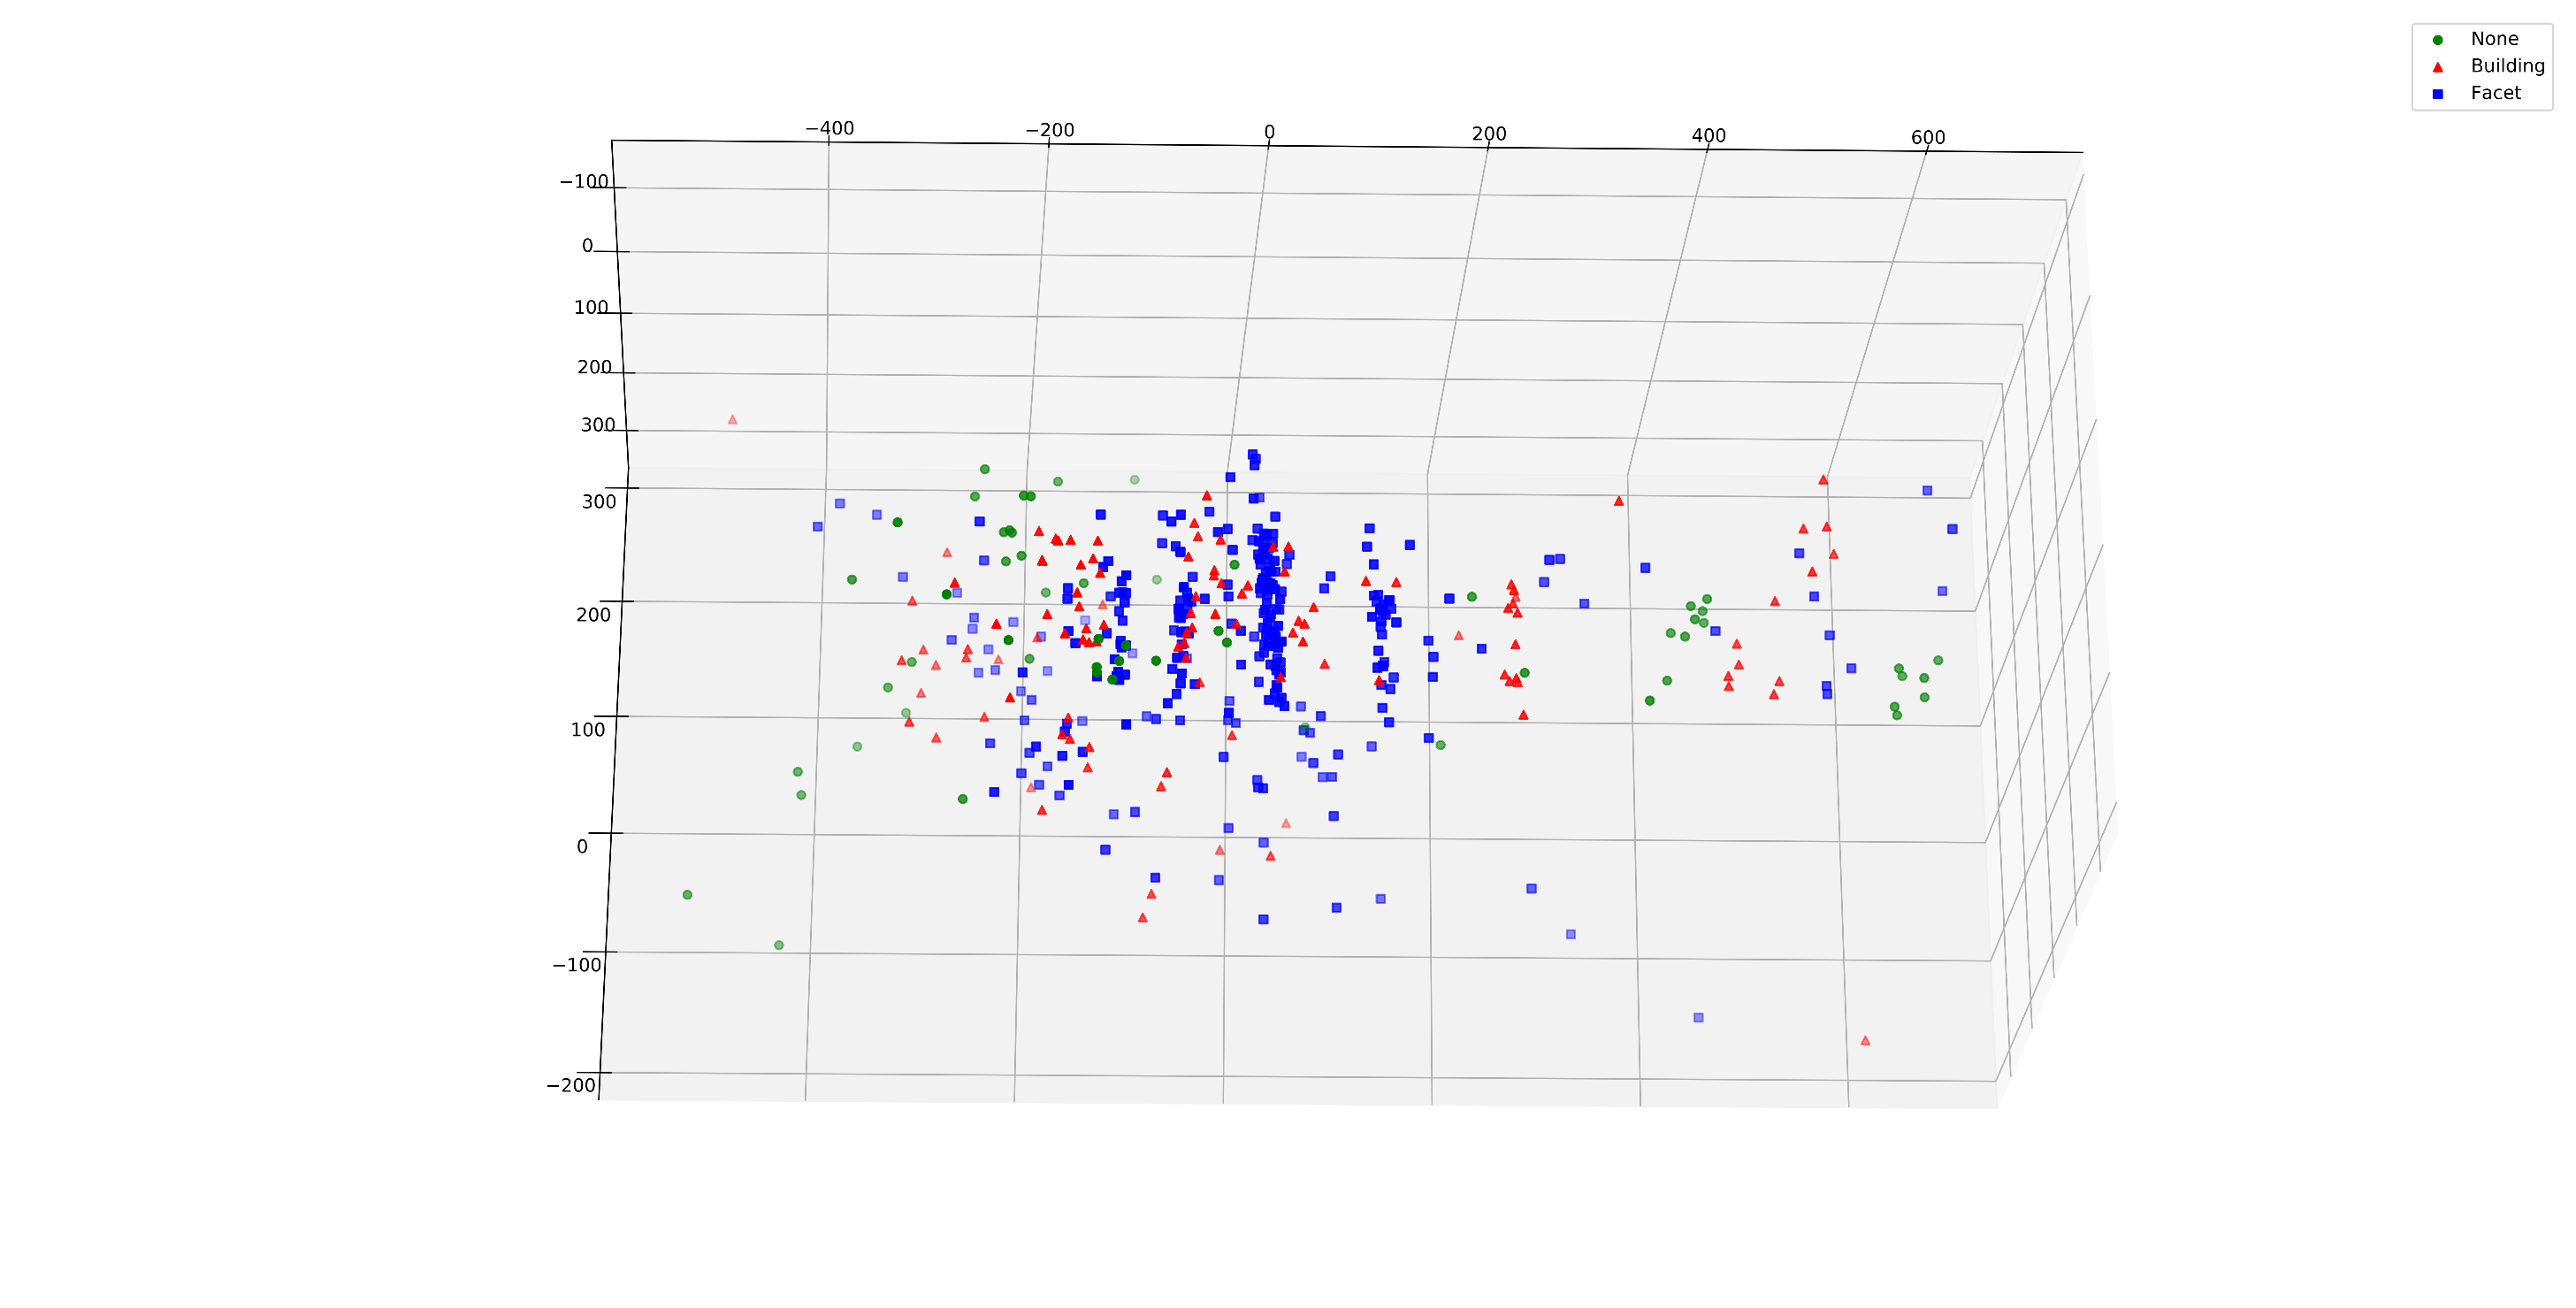
\includegraphics[width=.31\textwidth]{../images/vizualization/geom_feat_1.eps}}
                    }
                    {
                        \caption{We can see strips like structure of data.}\label{fig::geom_1}
                    }
                    \ffigbox[\FBwidth]
                    {
                        \fbox{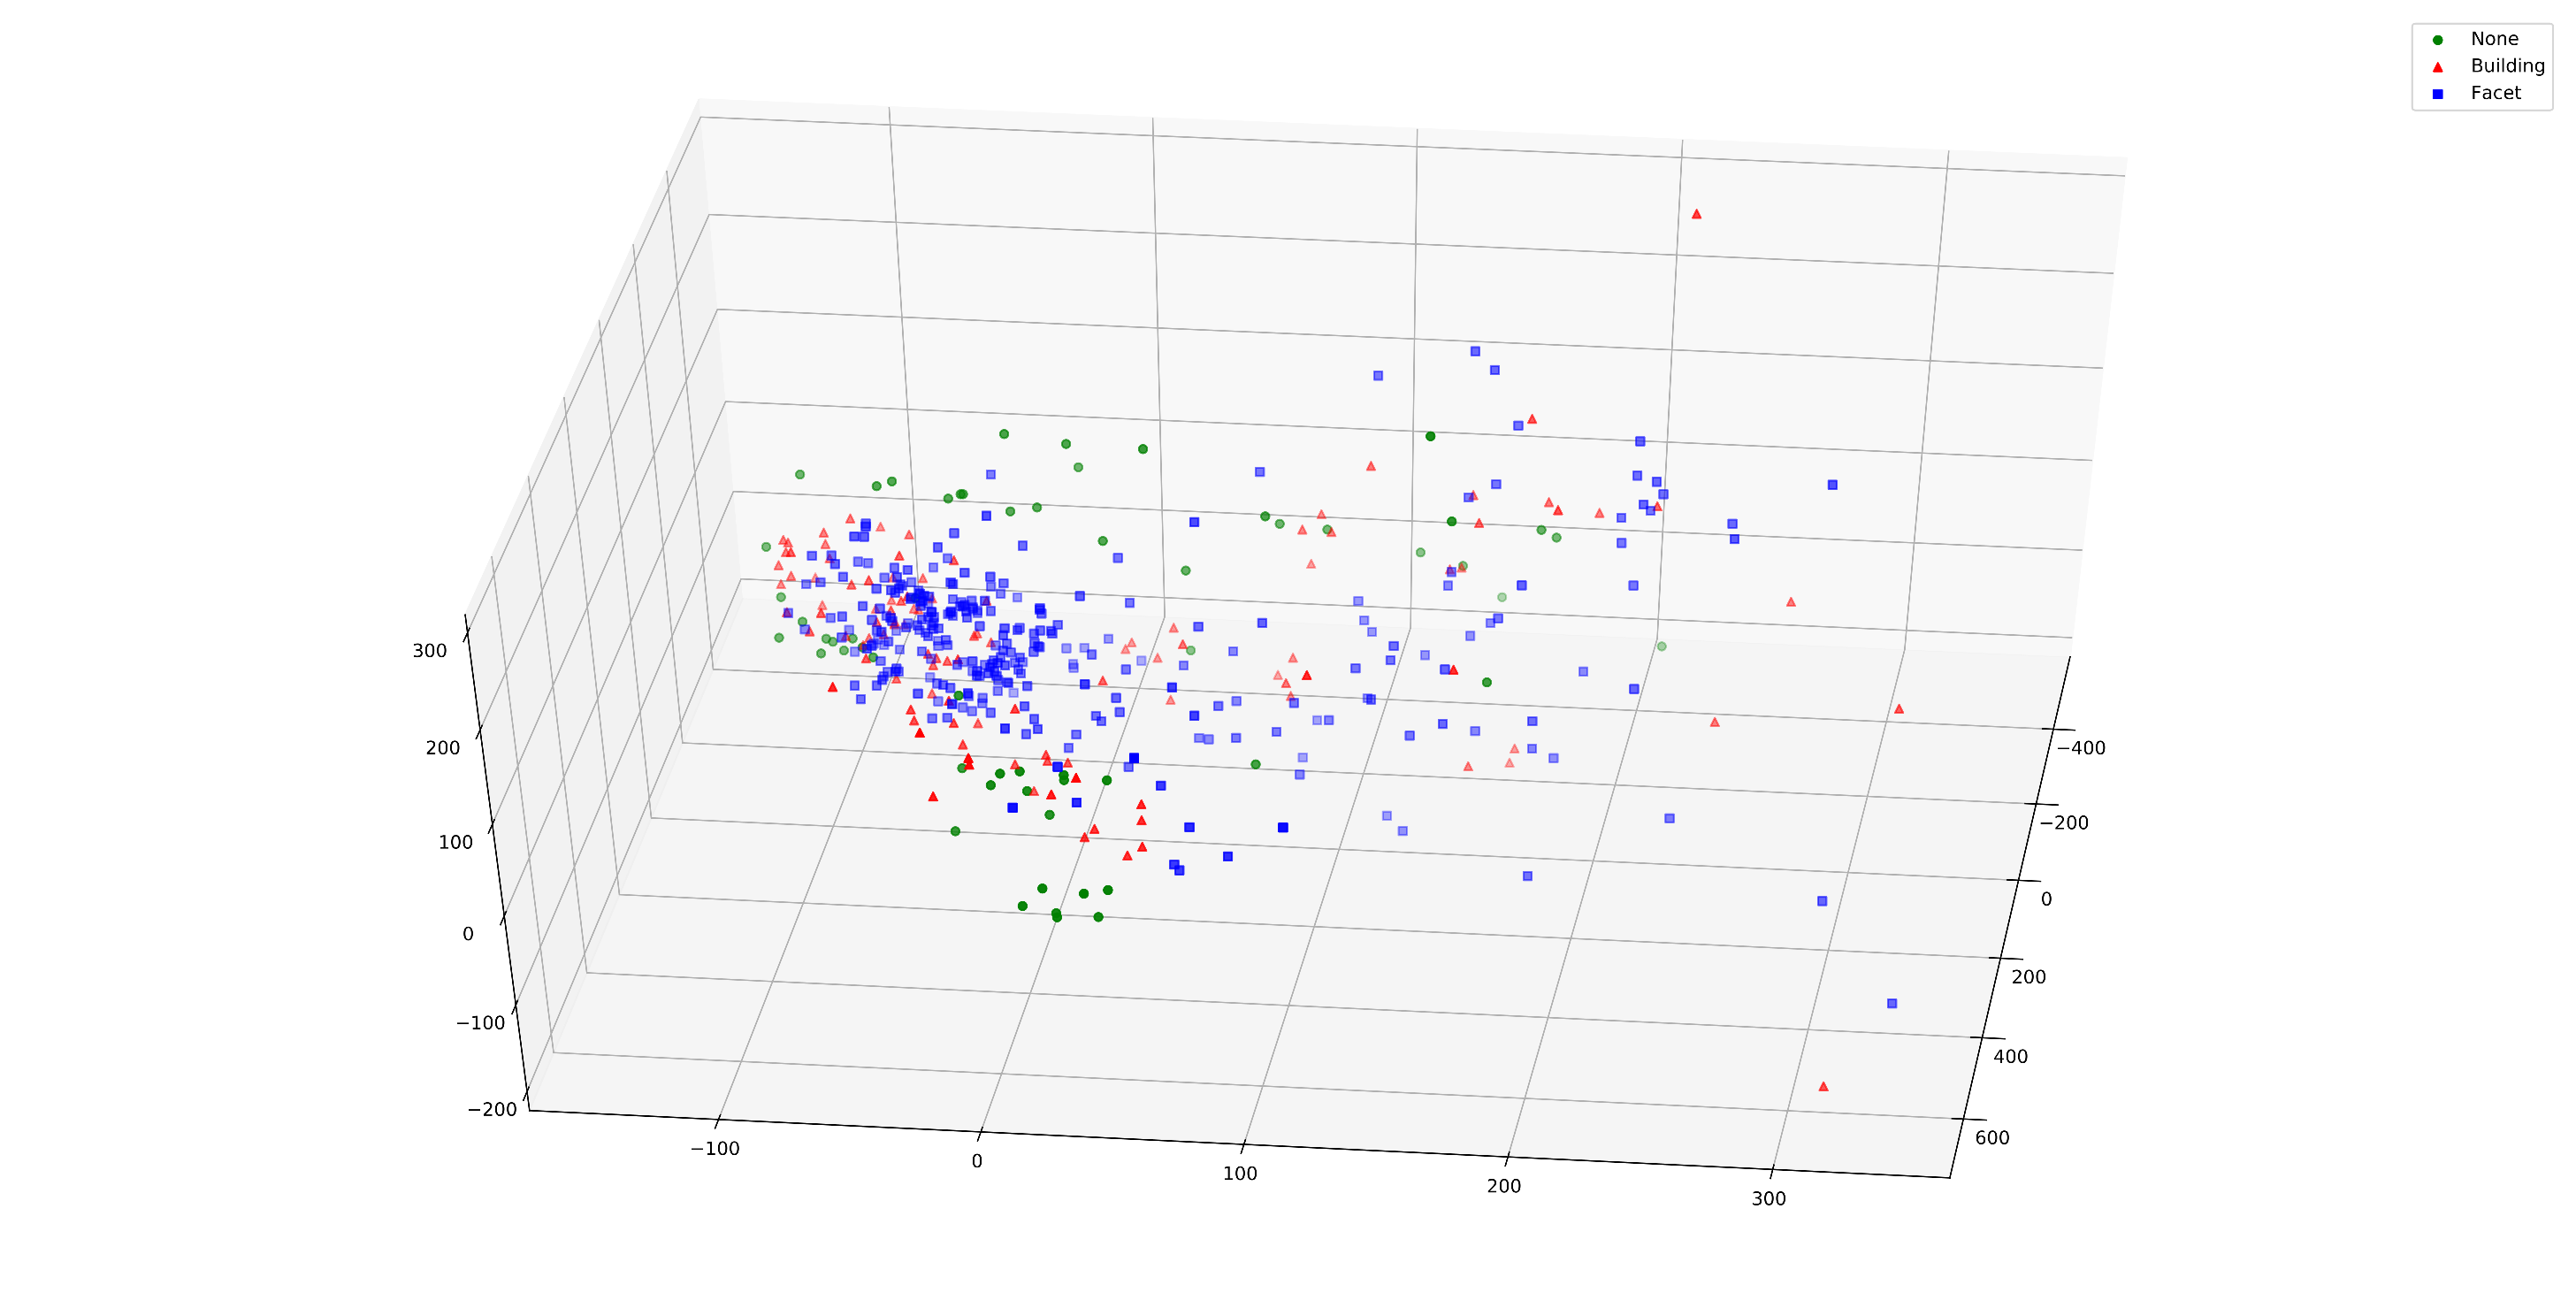
\includegraphics[width=.31\textwidth]{../images/vizualization/geom_feat_2.eps}}
                    }
                    {
                        \caption{We cannot see much in this direction.}\label{fig::geom_2}
                    }
                    \ffigbox[\FBwidth]
                    {
                        \fbox{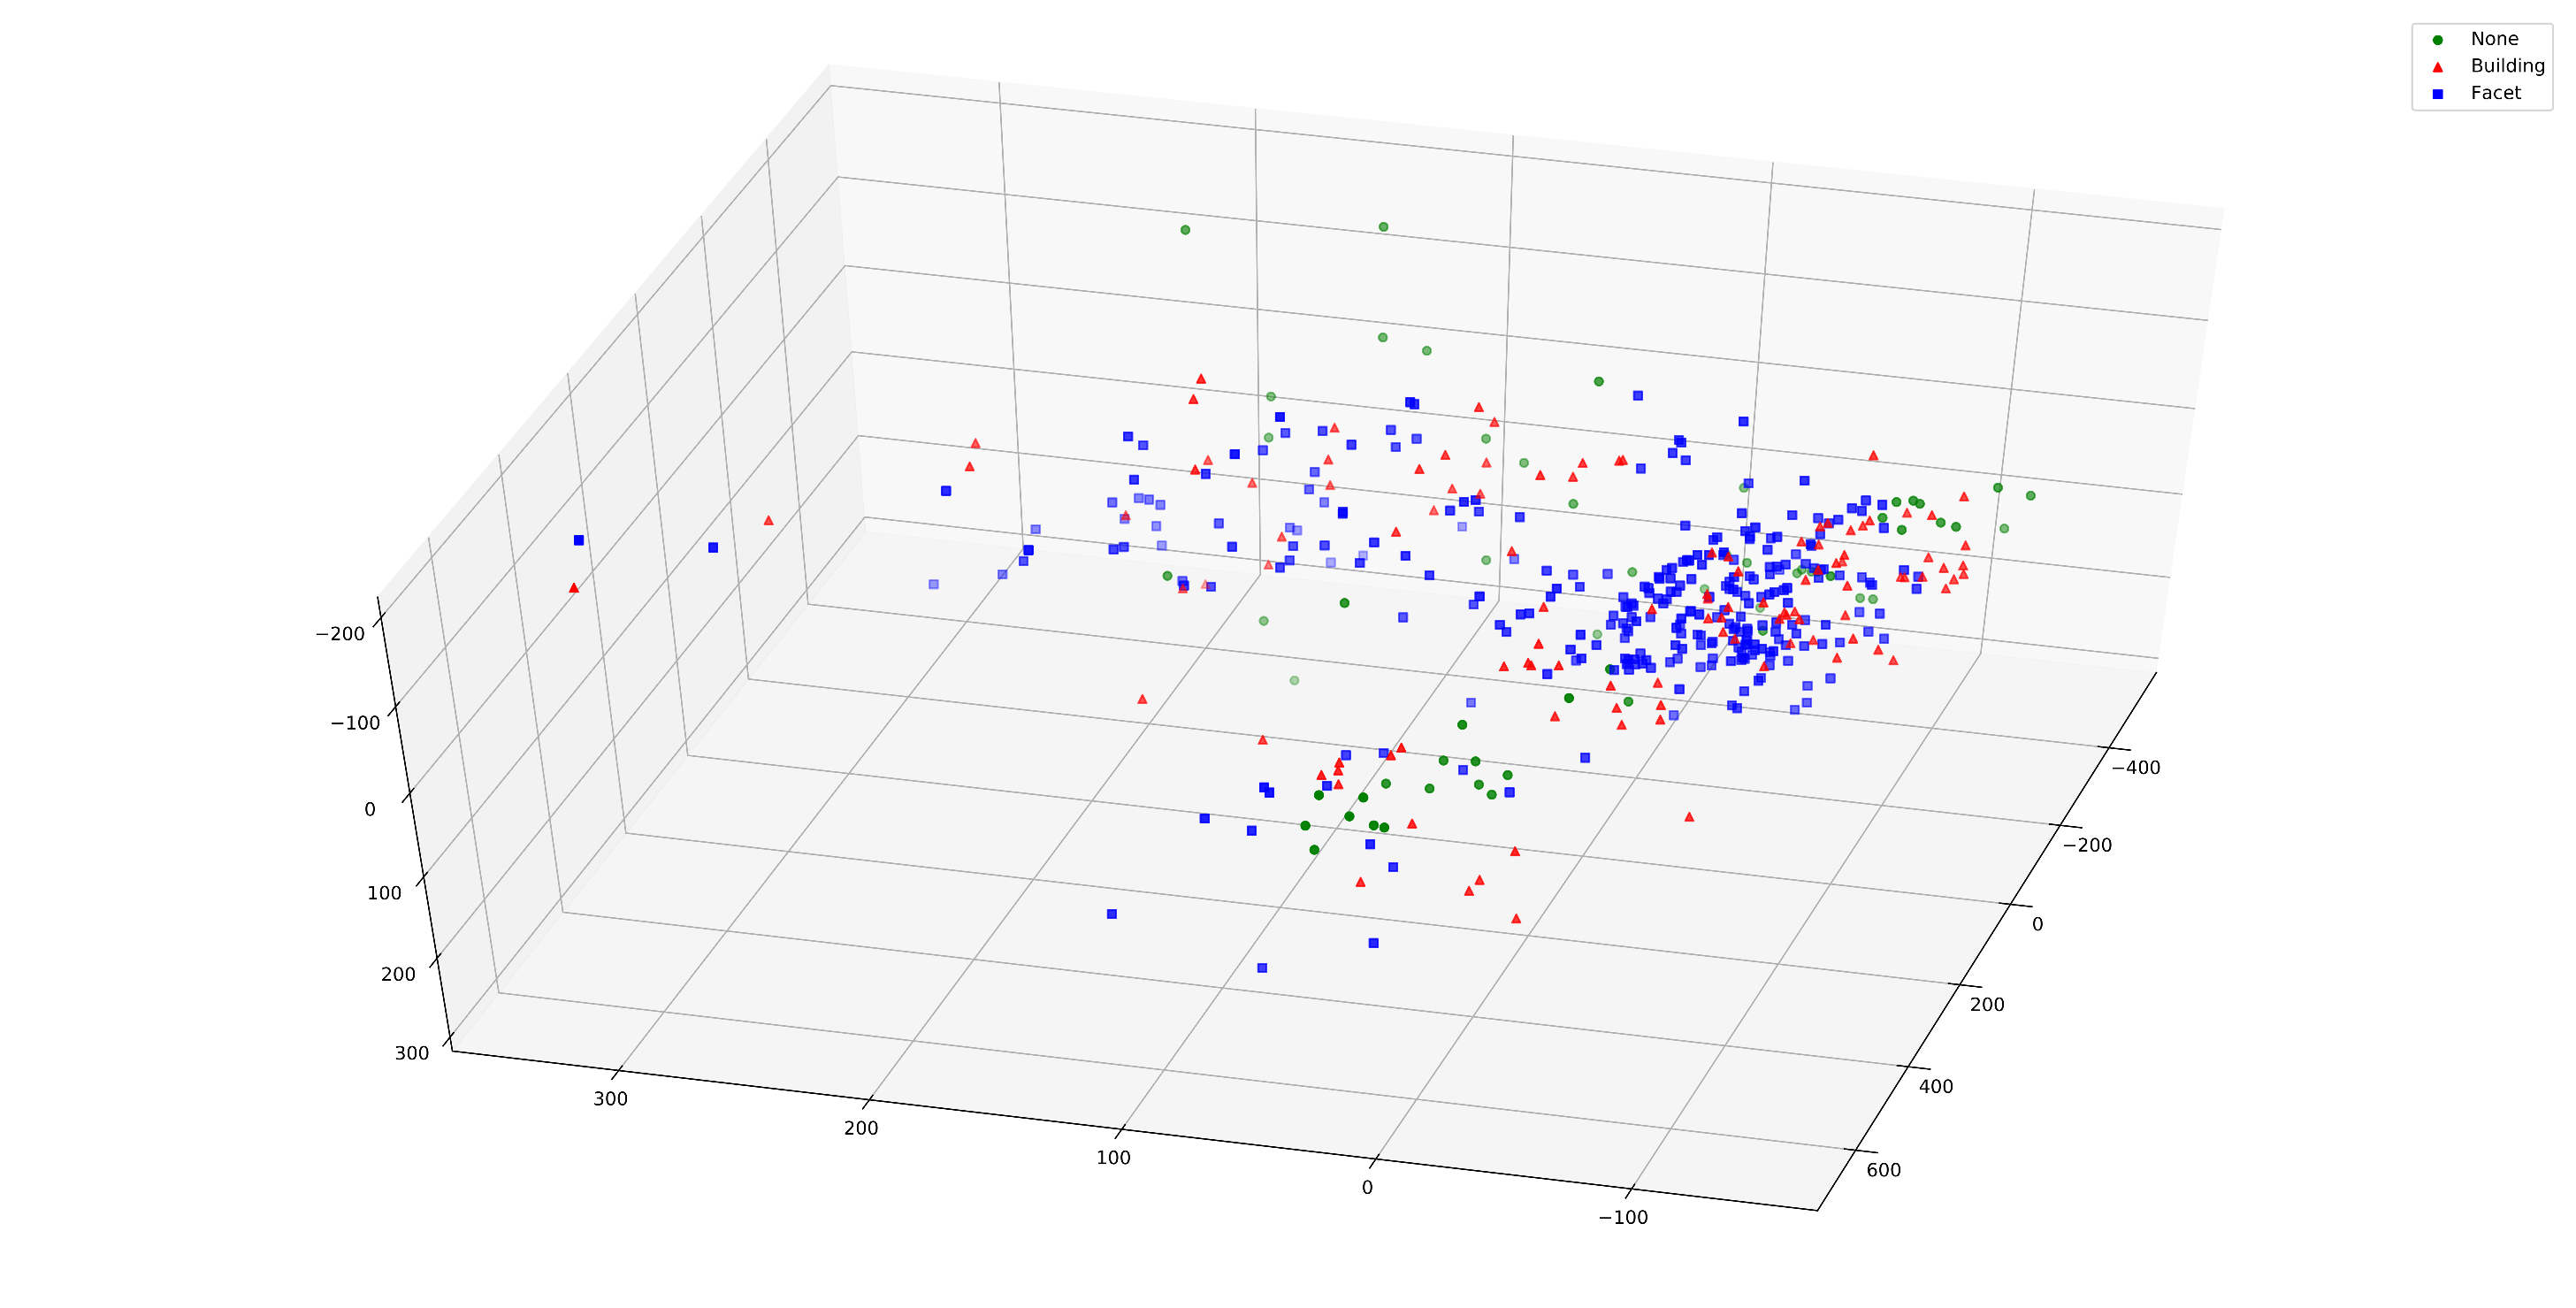
\includegraphics[width=.31\textwidth]{../images/vizualization/geom_feat_3.eps}}
                    }
                    {
                        \caption{We can observe some local structures but nothing global.}\label{fig::geom_3}
                    }
                \end{subfloatrow}
            }
            {
                \caption*{(i). Visualization of geometric features.}
            }
            \ffigbox[\FBwidth]
            {
                \begin{subfloatrow}[3]
                    \captionsetup{labelformat=brace, justification=raggedright}
                    \ffigbox[\FBwidth]
                    {
                        \fbox{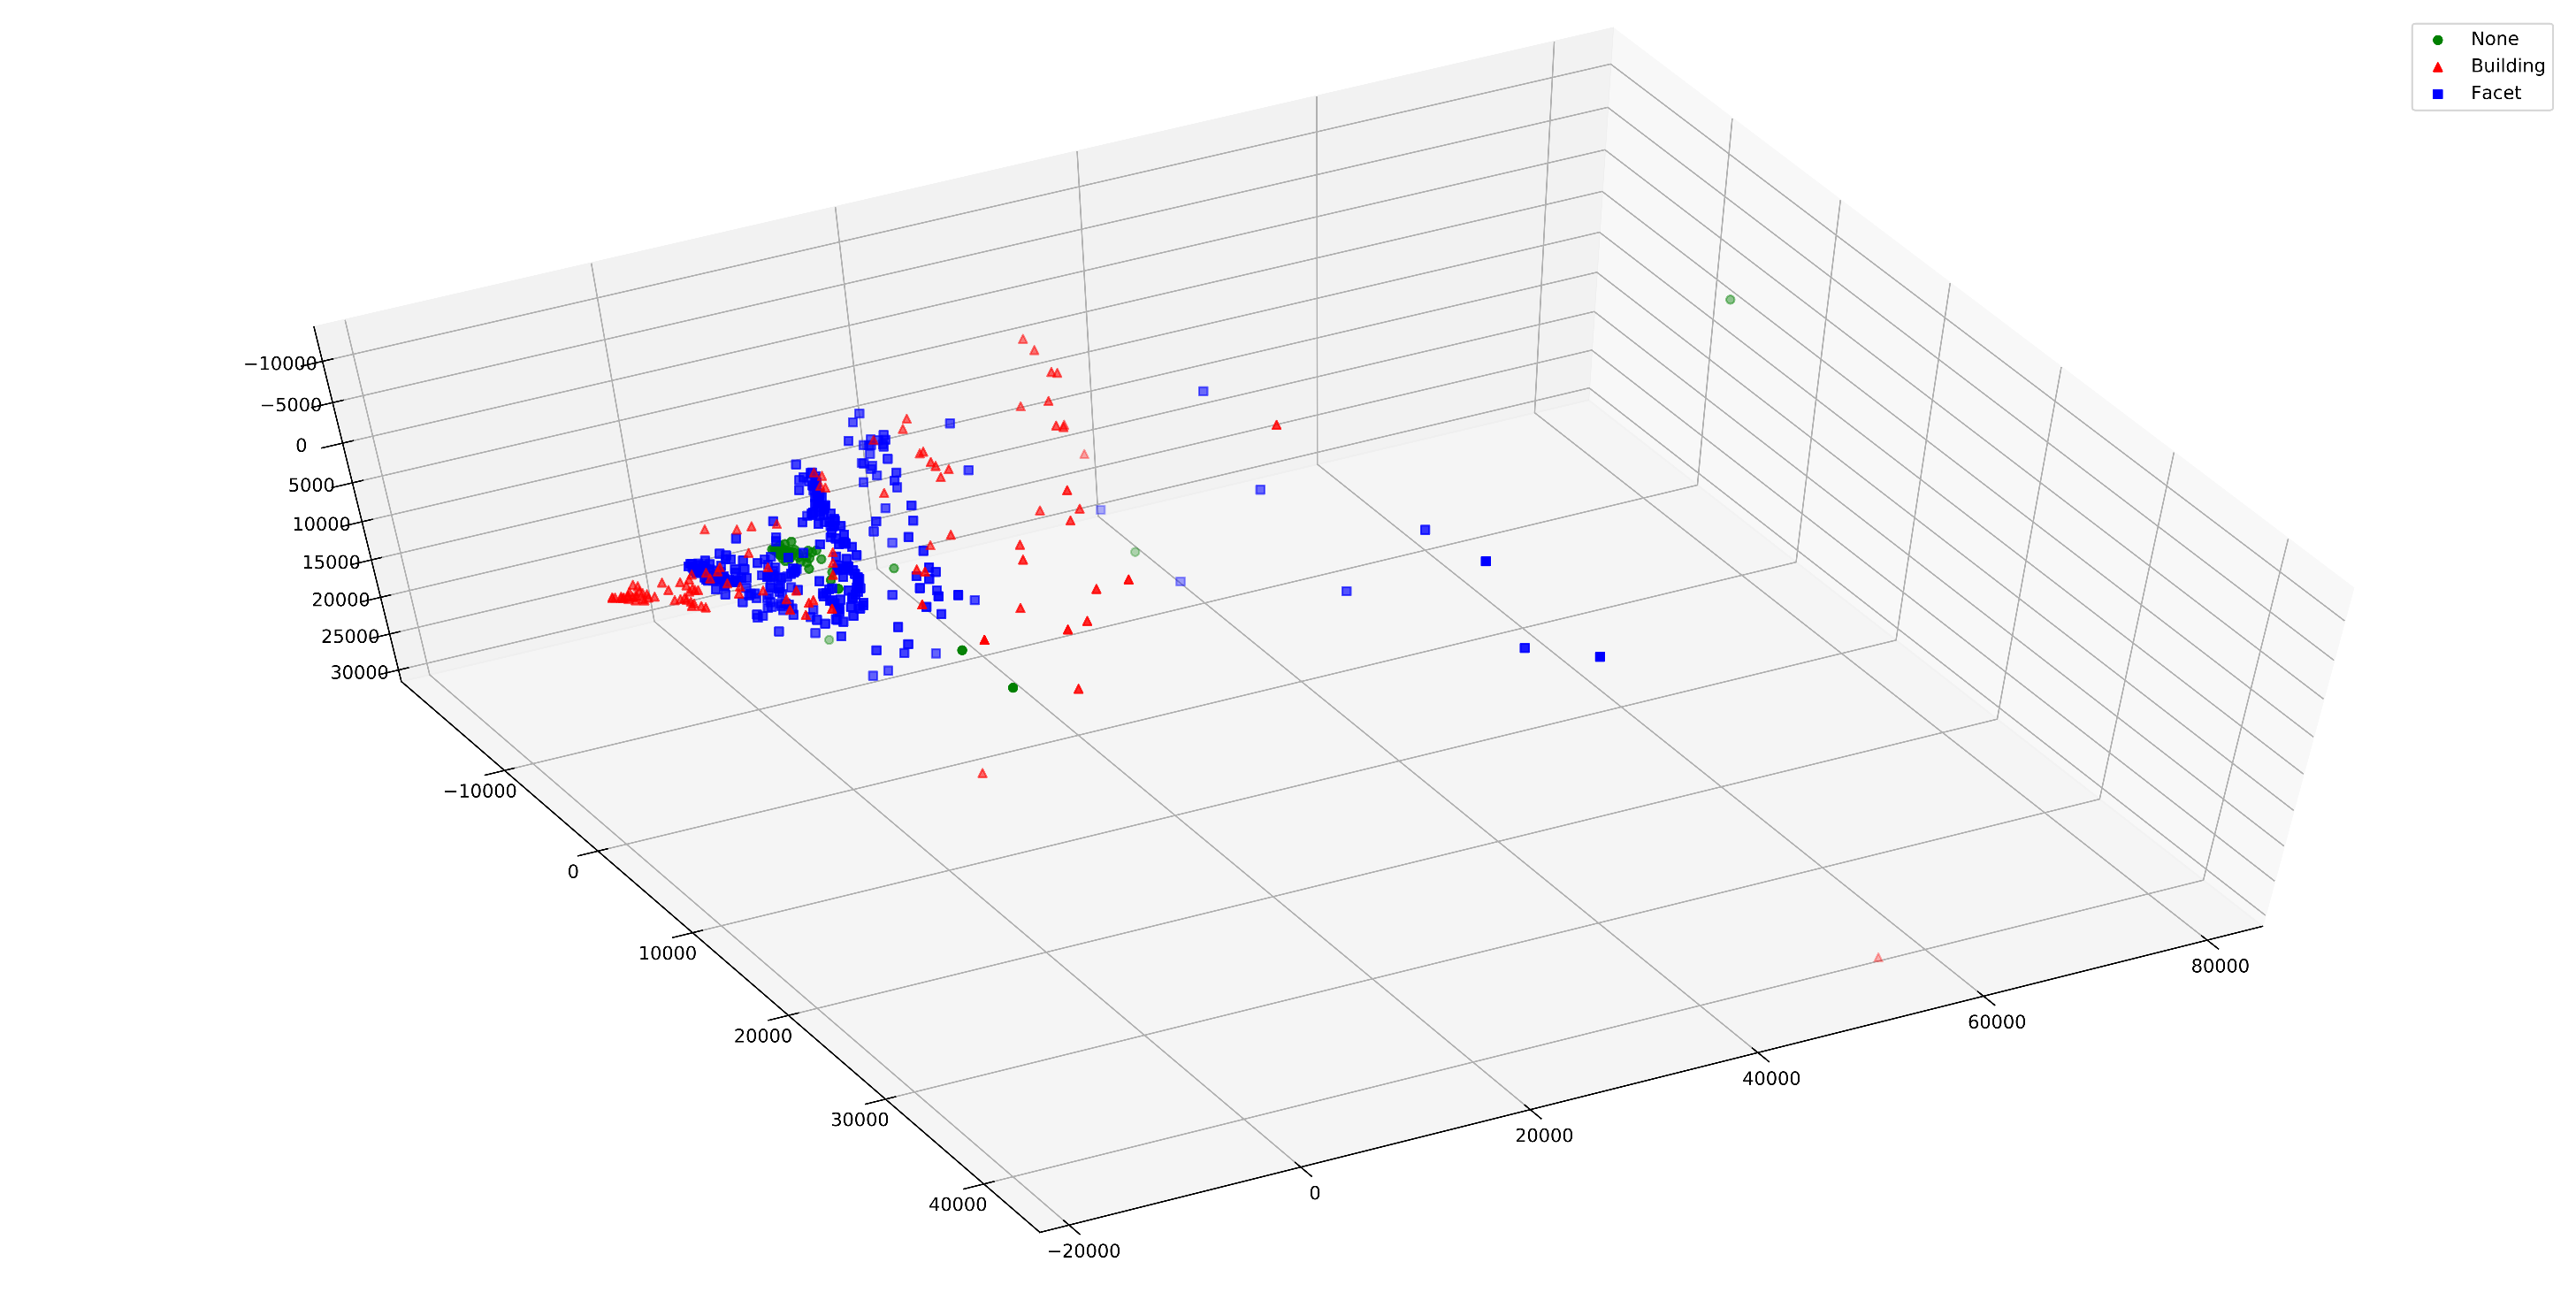
\includegraphics[width=.31\textwidth]{../images/vizualization/alti_feat_1.eps}}
                    }
                    {
                        \caption{We can see how the classes are disposed in halo like structures.}\label{fig::alti_1}
                    }
                    \ffigbox[\FBwidth]
                    {
                        \fbox{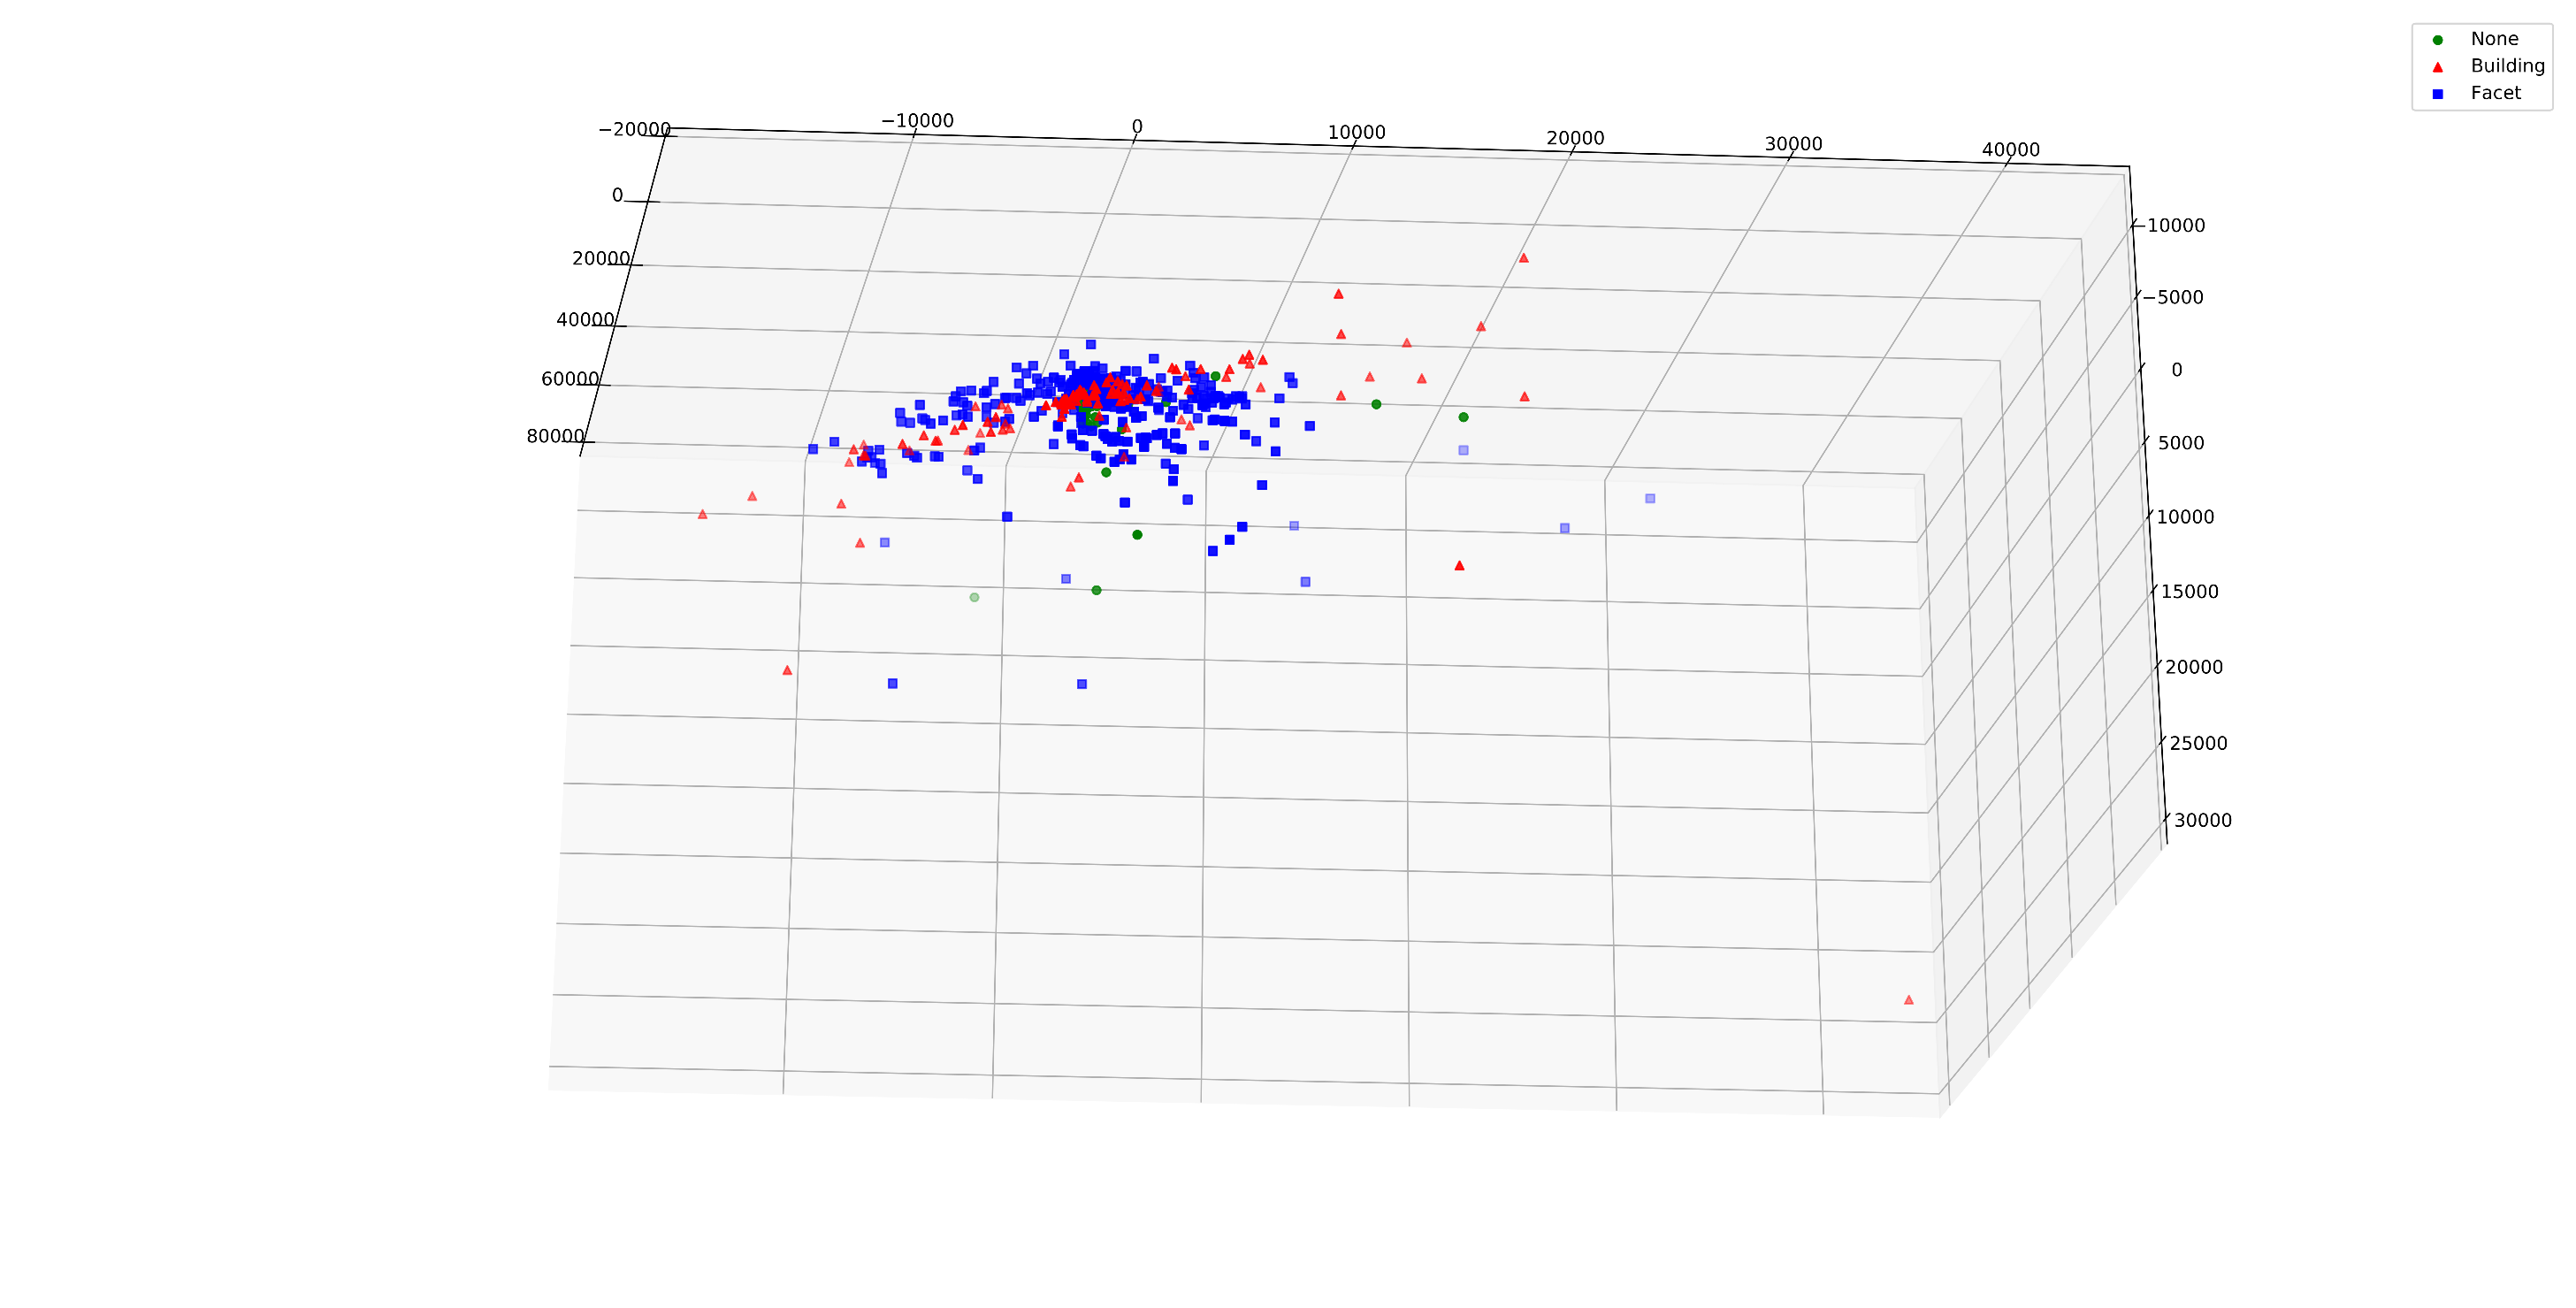
\includegraphics[width=.31\textwidth]{../images/vizualization/alti_feat_2.eps}}
                    }
                    {
                        \caption{This take confirms the fact that `None' errors are in the center followed by `Facet' errors and `Building' erros at last.}\label{fig::alti_2}
                    }
                    \ffigbox[\FBwidth]
                    {
                        \fbox{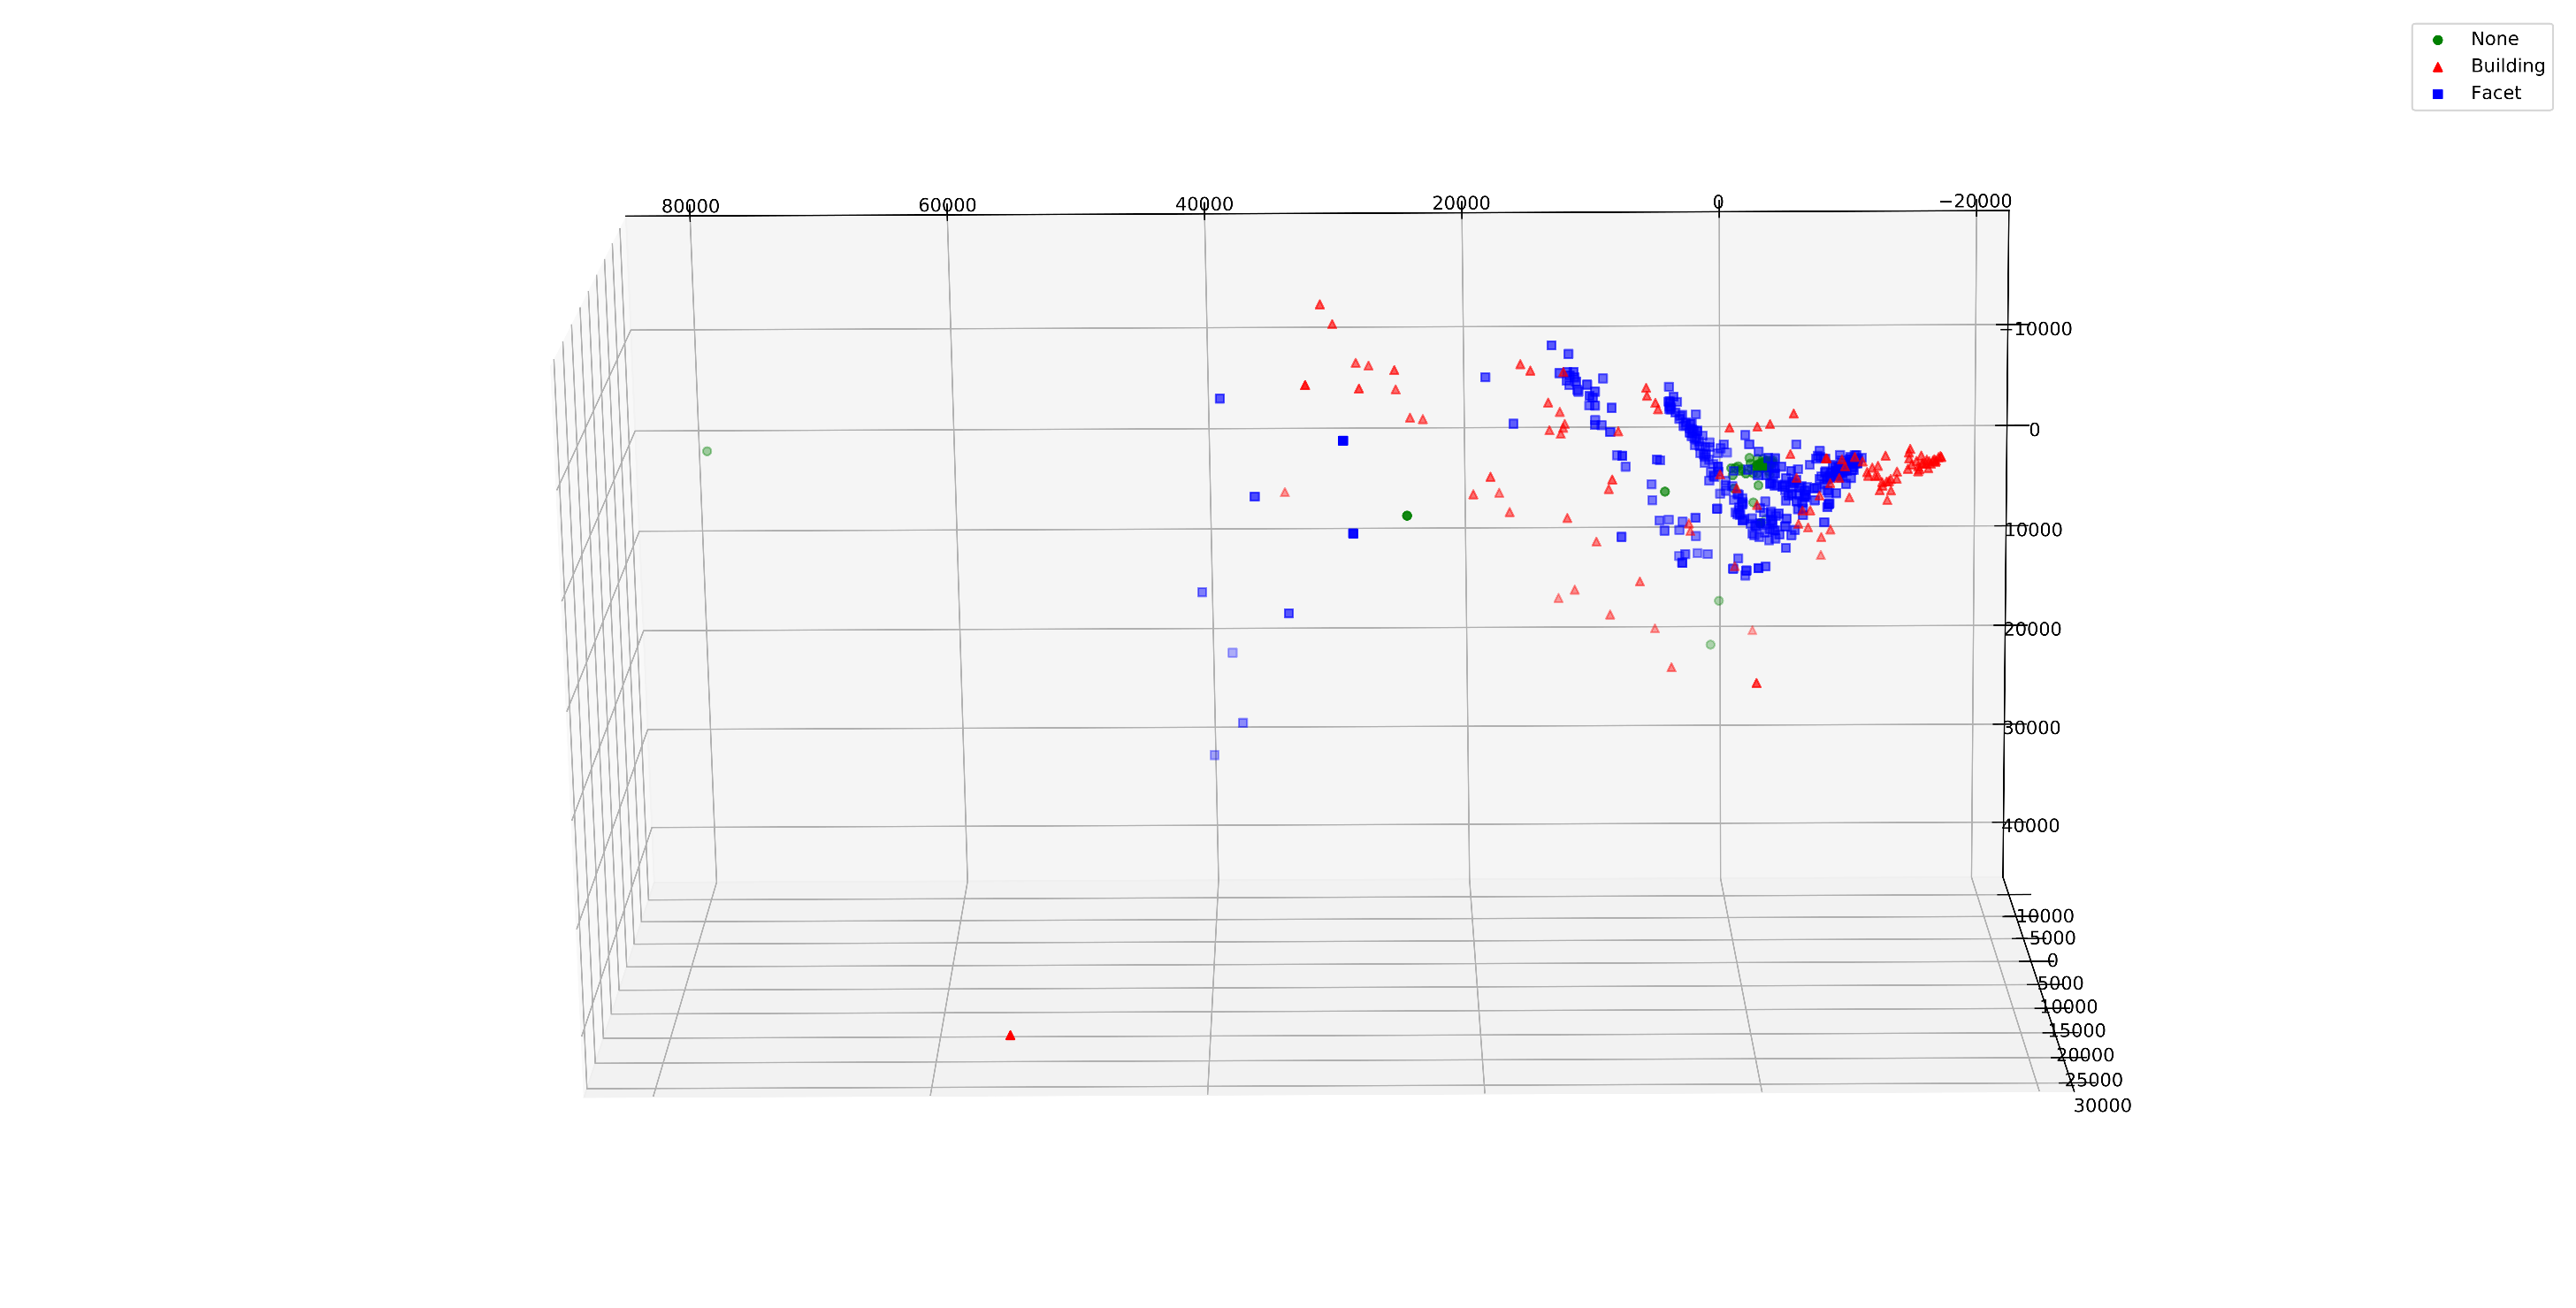
\includegraphics[width=.31\textwidth]{../images/vizualization/alti_feat_3.eps}}
                    }
                    {
                        \caption{We can see clearly the halo like structures.}\label{fig::alti_3}
                    }
                \end{subfloatrow}
            }
            {
                \renewcommand\figurename{}
                \renewcommand{\thefigure}{(\roman{SubFigCounter})}

                \caption{Visualization of altimetric features.}\label{fig::alt_viz}
                \refstepcounter{SubFigCounter}
            }
            \ffigbox[\FBwidth]
            {
                \begin{subfloatrow}[3]
                    \captionsetup{labelformat=brace, justification=raggedright}
                    \ffigbox[\FBwidth]
                    {
                        \fbox{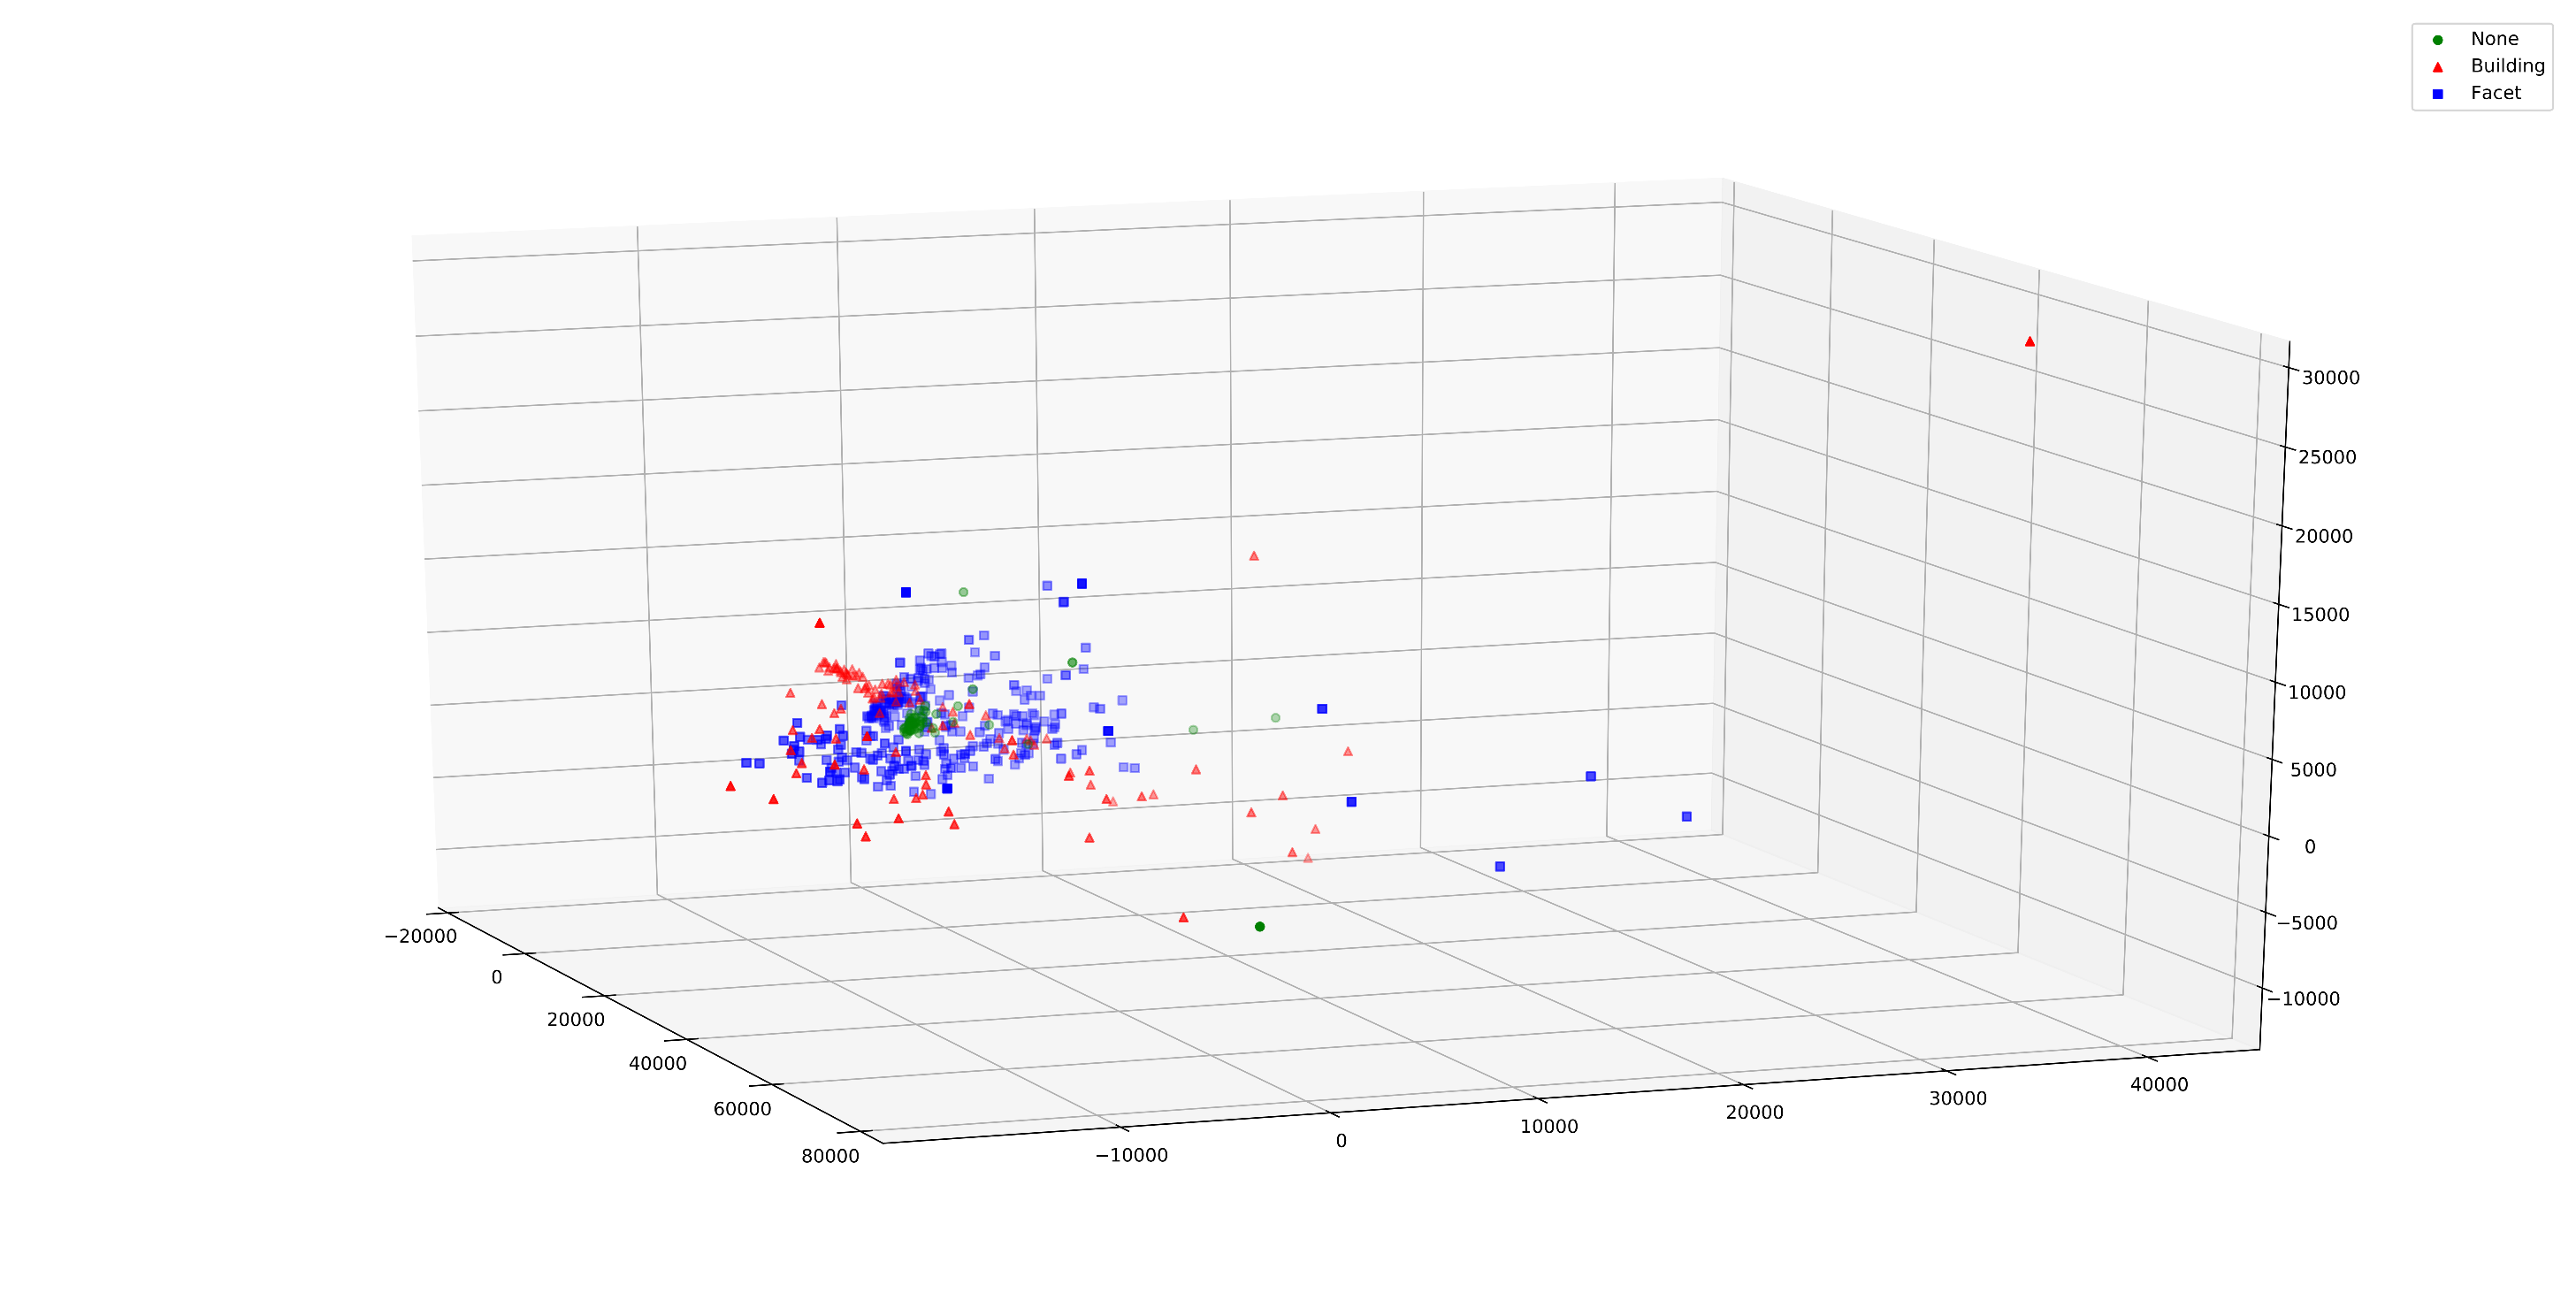
\includegraphics[width=.31\textwidth]{../images/vizualization/fused_feat_1.eps}}
                    }
                    {
                        \caption{We keep the same disposition of classes as in altimetric features.}\label{fig::fused_1}
                    }
                    \ffigbox[\FBwidth]
                    {
                        \fbox{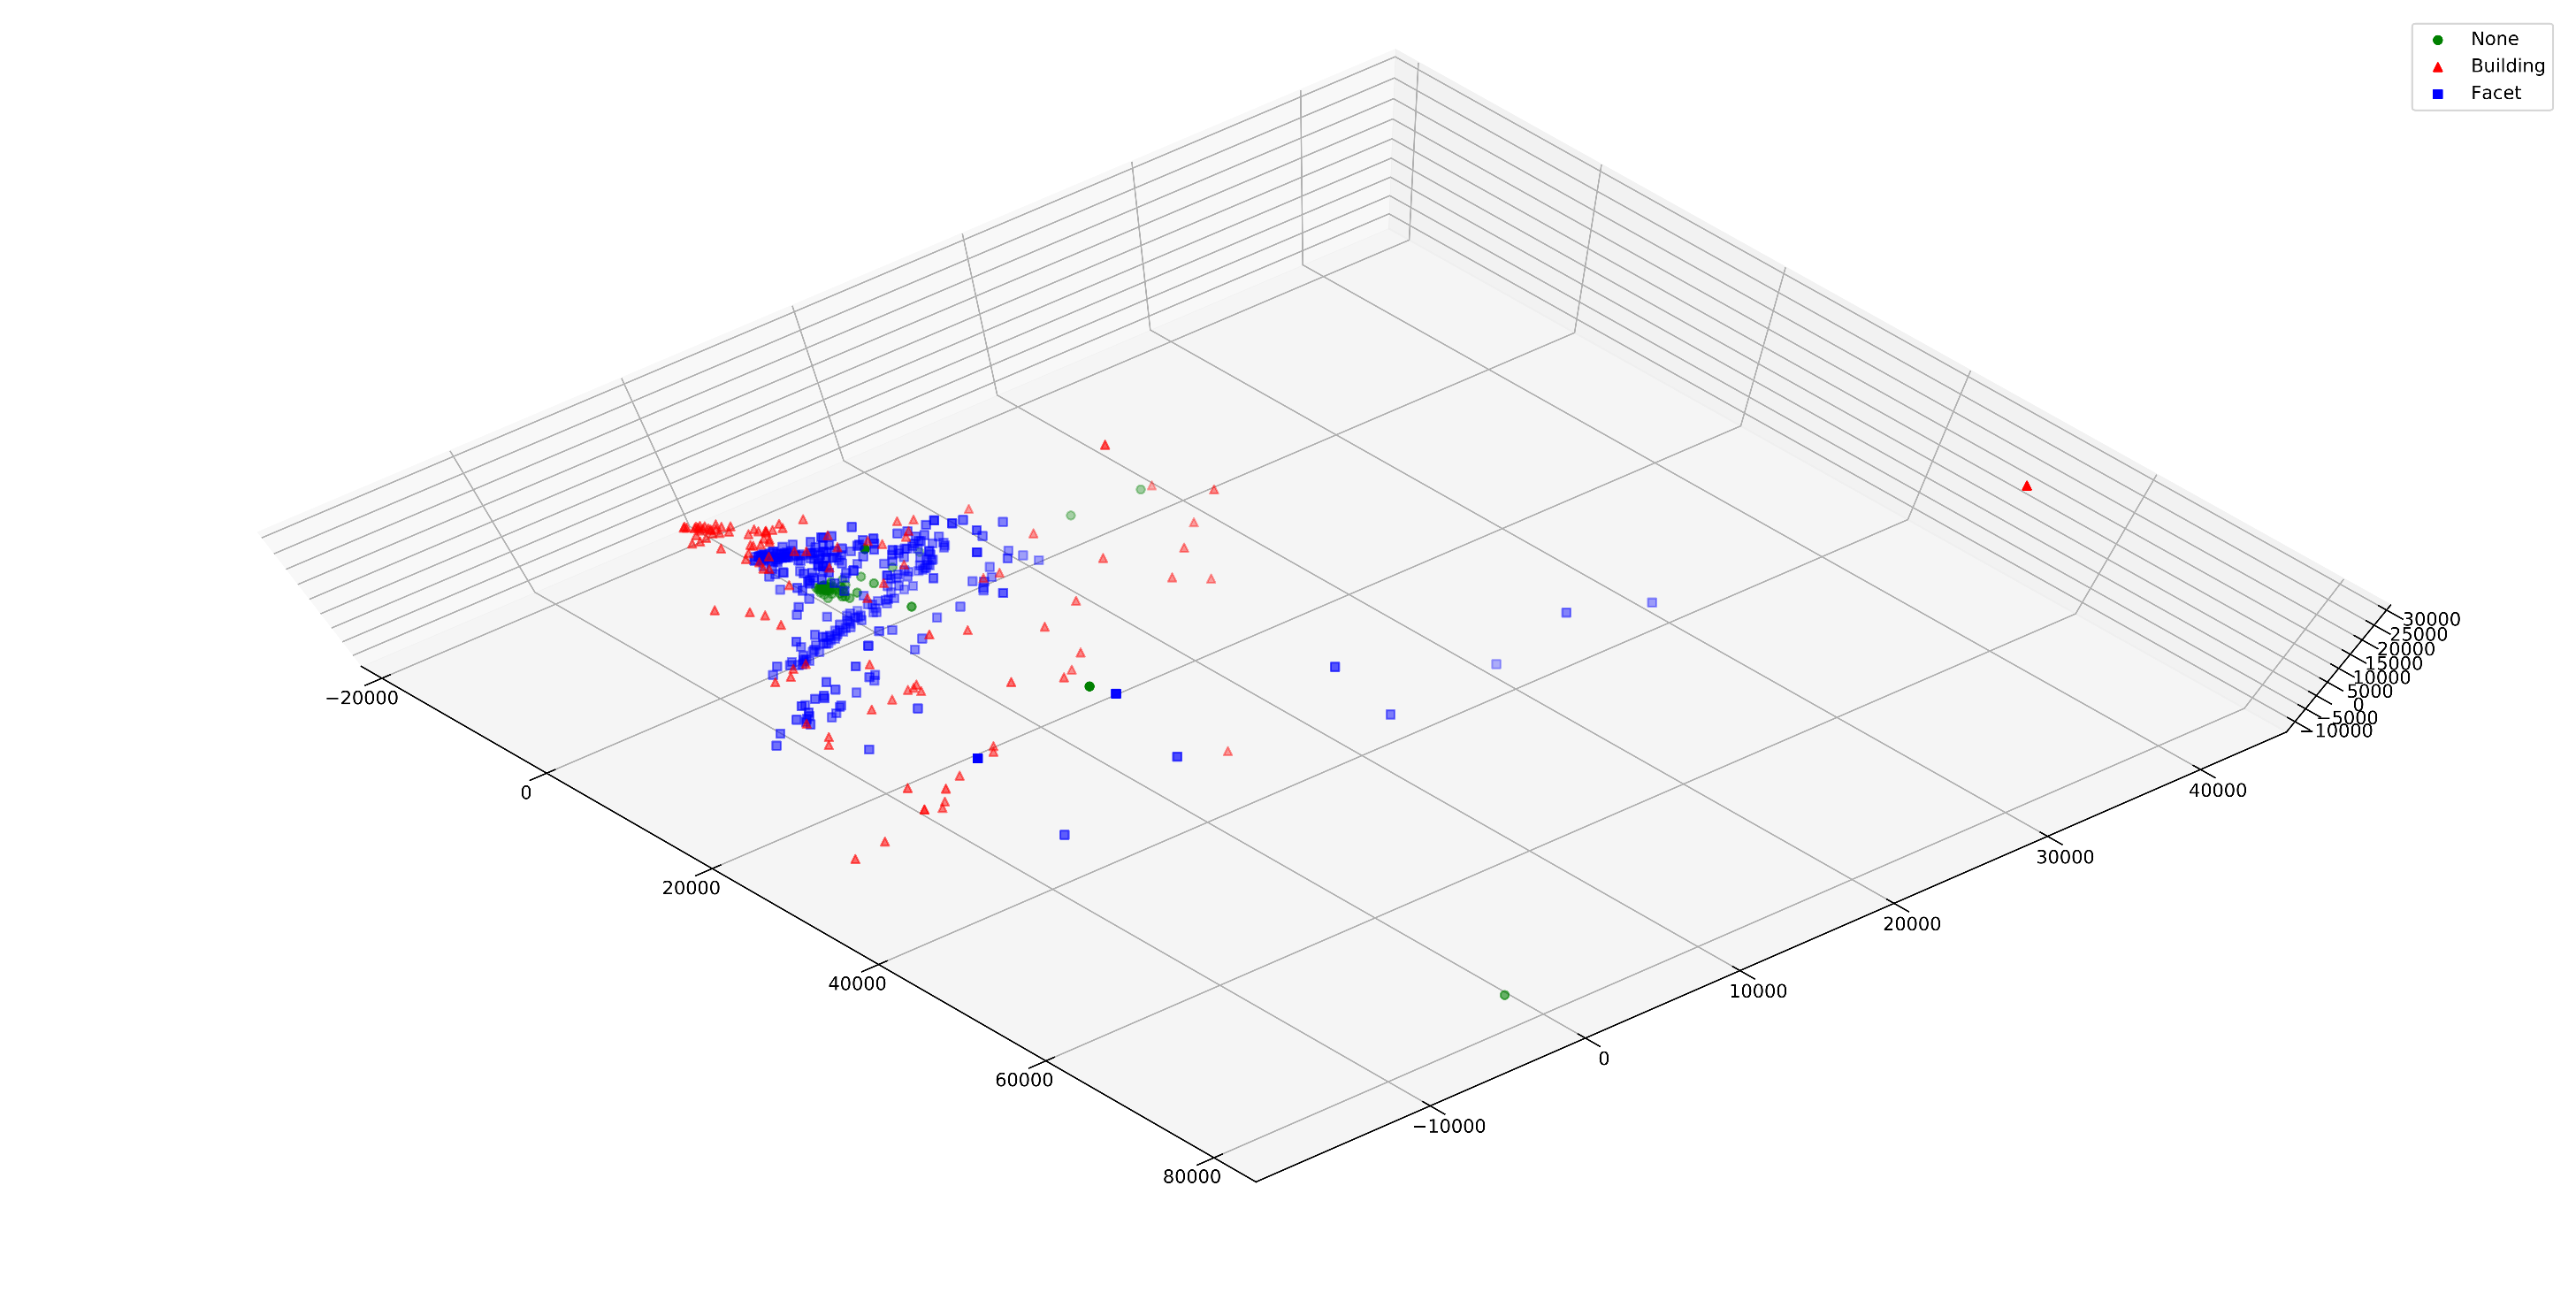
\includegraphics[width=.31\textwidth]{../images/vizualization/fused_feat_2.eps}}
                    }
                    {
                        \caption{The same halos as in Figure~\ref{fig::alt_viz}~\ref{fig::alti_3} but more compact.}\label{fig::fused_2}
                    }
                    \ffigbox[\FBwidth]
                    {
                        \fbox{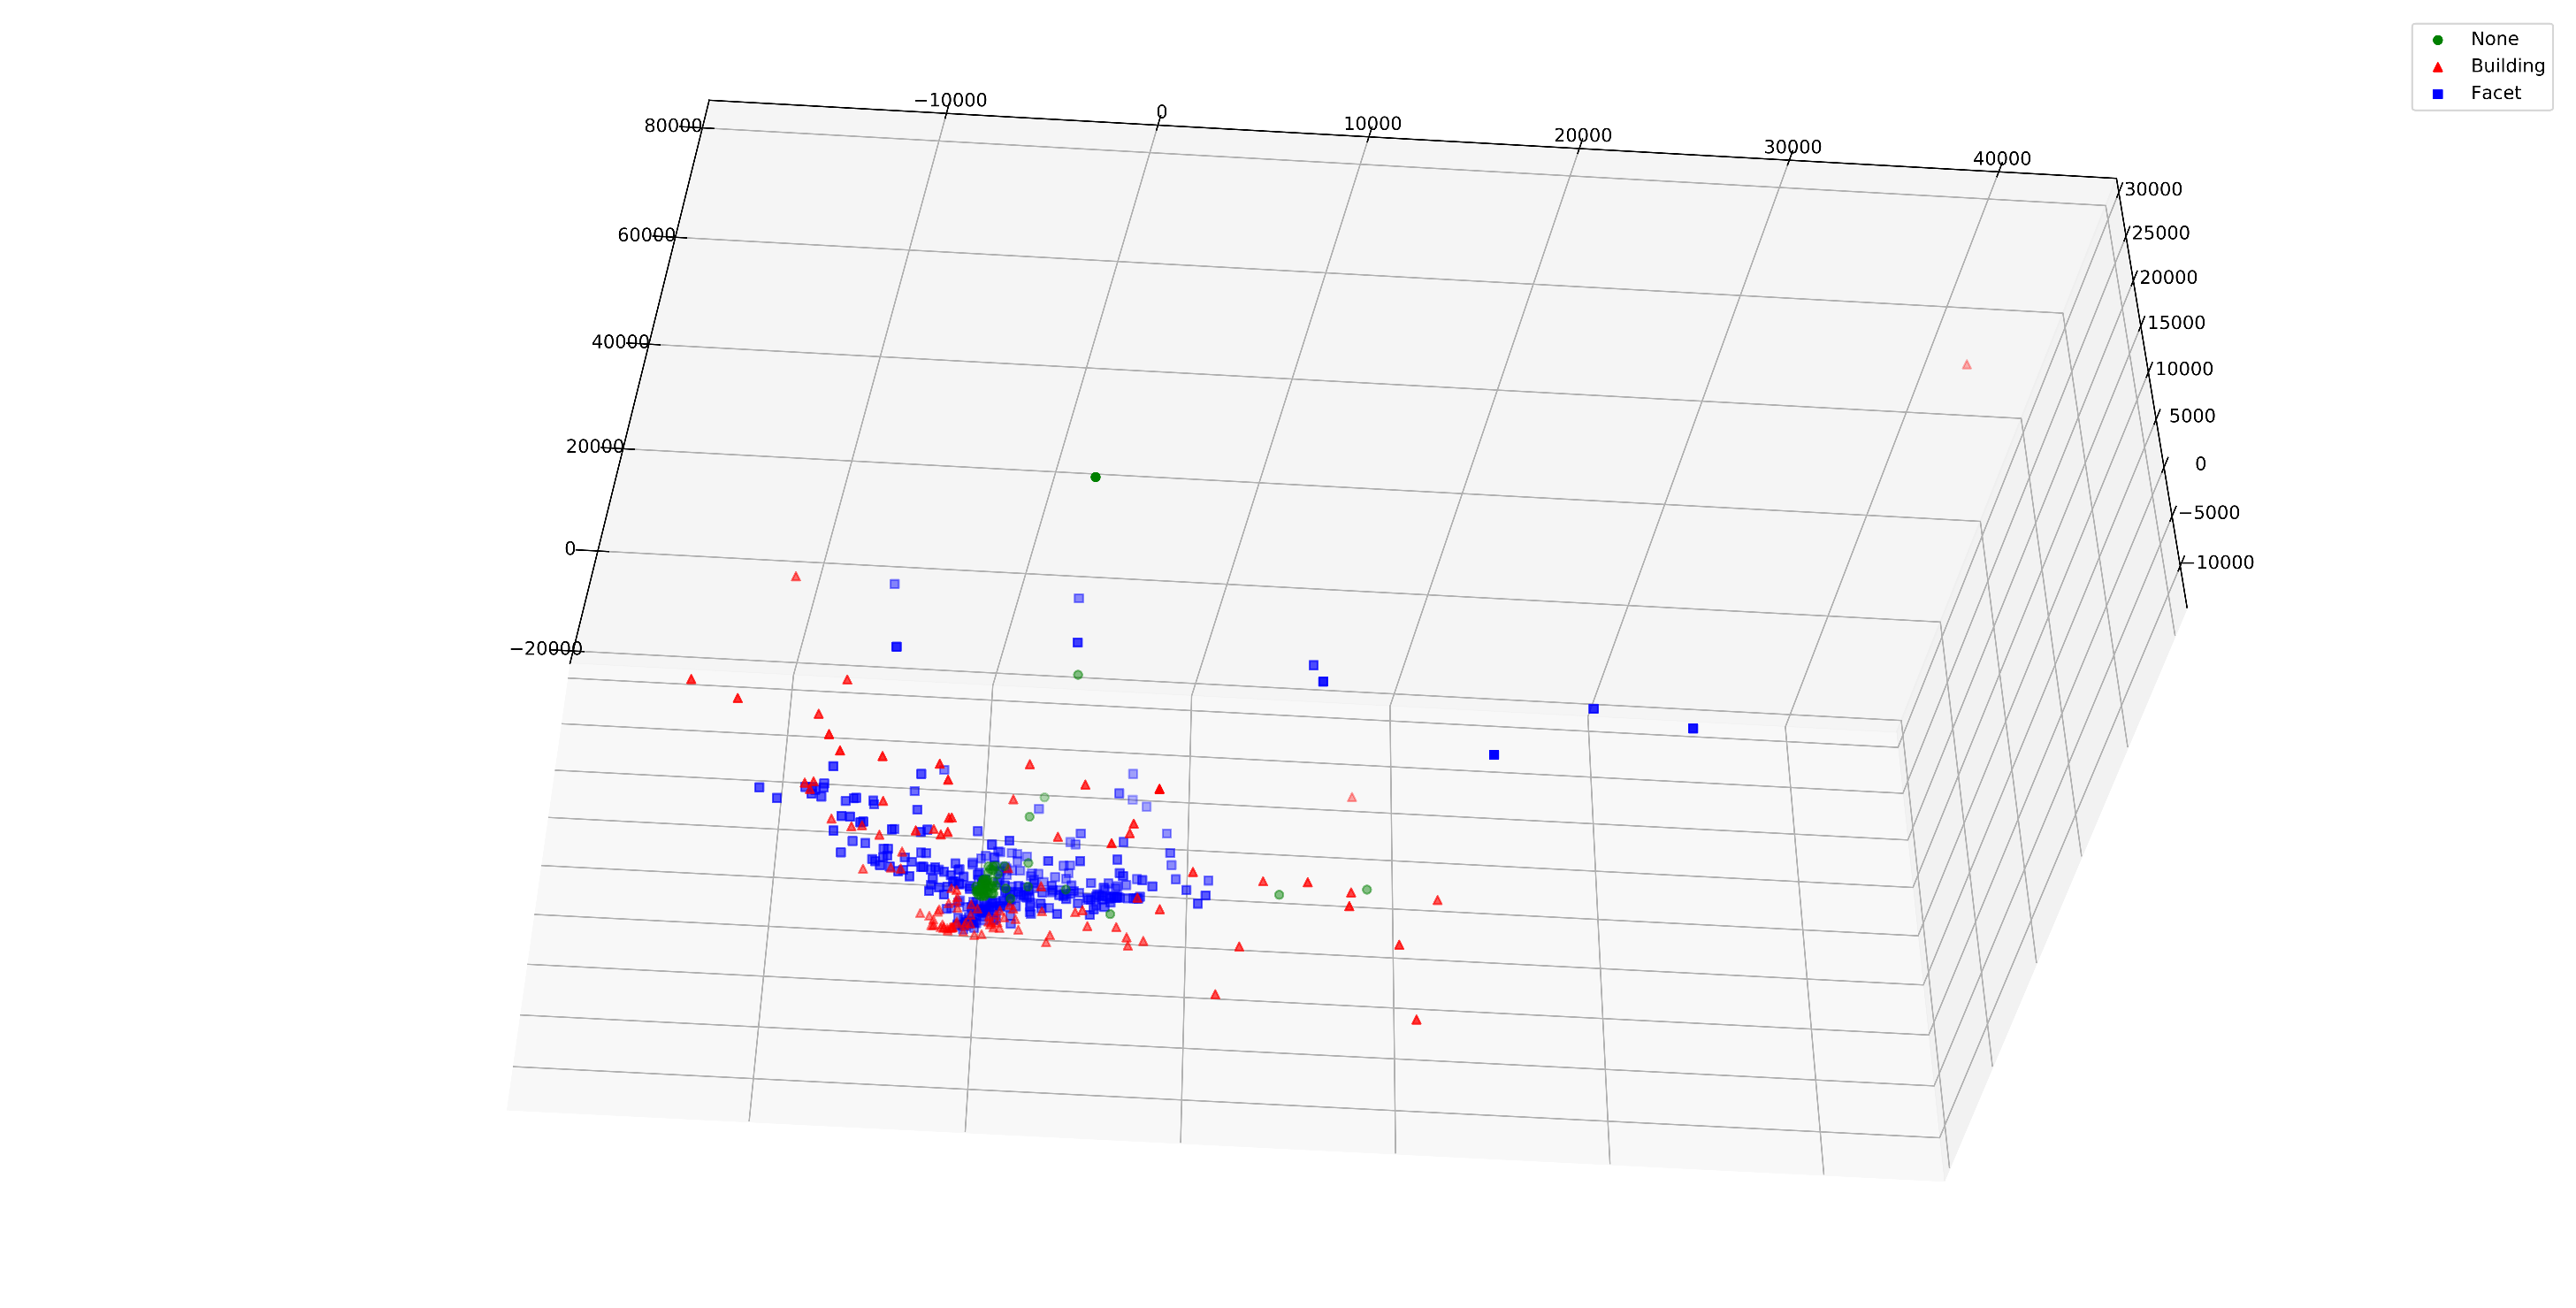
\includegraphics[width=.31\textwidth]{../images/vizualization/fused_feat_3.eps}}
                    }
                    {
                        \caption{The same forms as in Figure~\ref{fig::pca_viz} -- (ii) --~\ref{fig::alti_2}.}\label{fig::fused_3}
                    }
                \end{subfloatrow}
            }
            {
                \caption*{(iii). Visualization fused features.}
            }
        }
        {
            \caption{\label{fig::pca_viz} Visualization of \textit{PCA} reduced features.}
        }
    \end{figure}

    I am trying also to cluster the features in between $9$ --- number of all subclasses --- and $3$ --- number of Coarse classes --- clusters. The idea is to see if features can be interpreted and are well defined or we are overfitting during classification. In Figure~\ref{fig::clust_viz}, we choose 7 clusters. The outliers cause both methods to have clusters with only one element, but otherwise we can see how it can capture coarse structures in data that do not correspond always to defined classes.

    \thisfloatsetup{heightadjust=object}
    \begin{figure}[H]
        \ffigbox{
            \ffigbox[\FBwidth]{
                \begin{subfloatrow}[2]
                    \captionsetup{labelformat=brace, justification=raggedright}
                    \ffigbox[\FBwidth]
                    {
                        \fbox{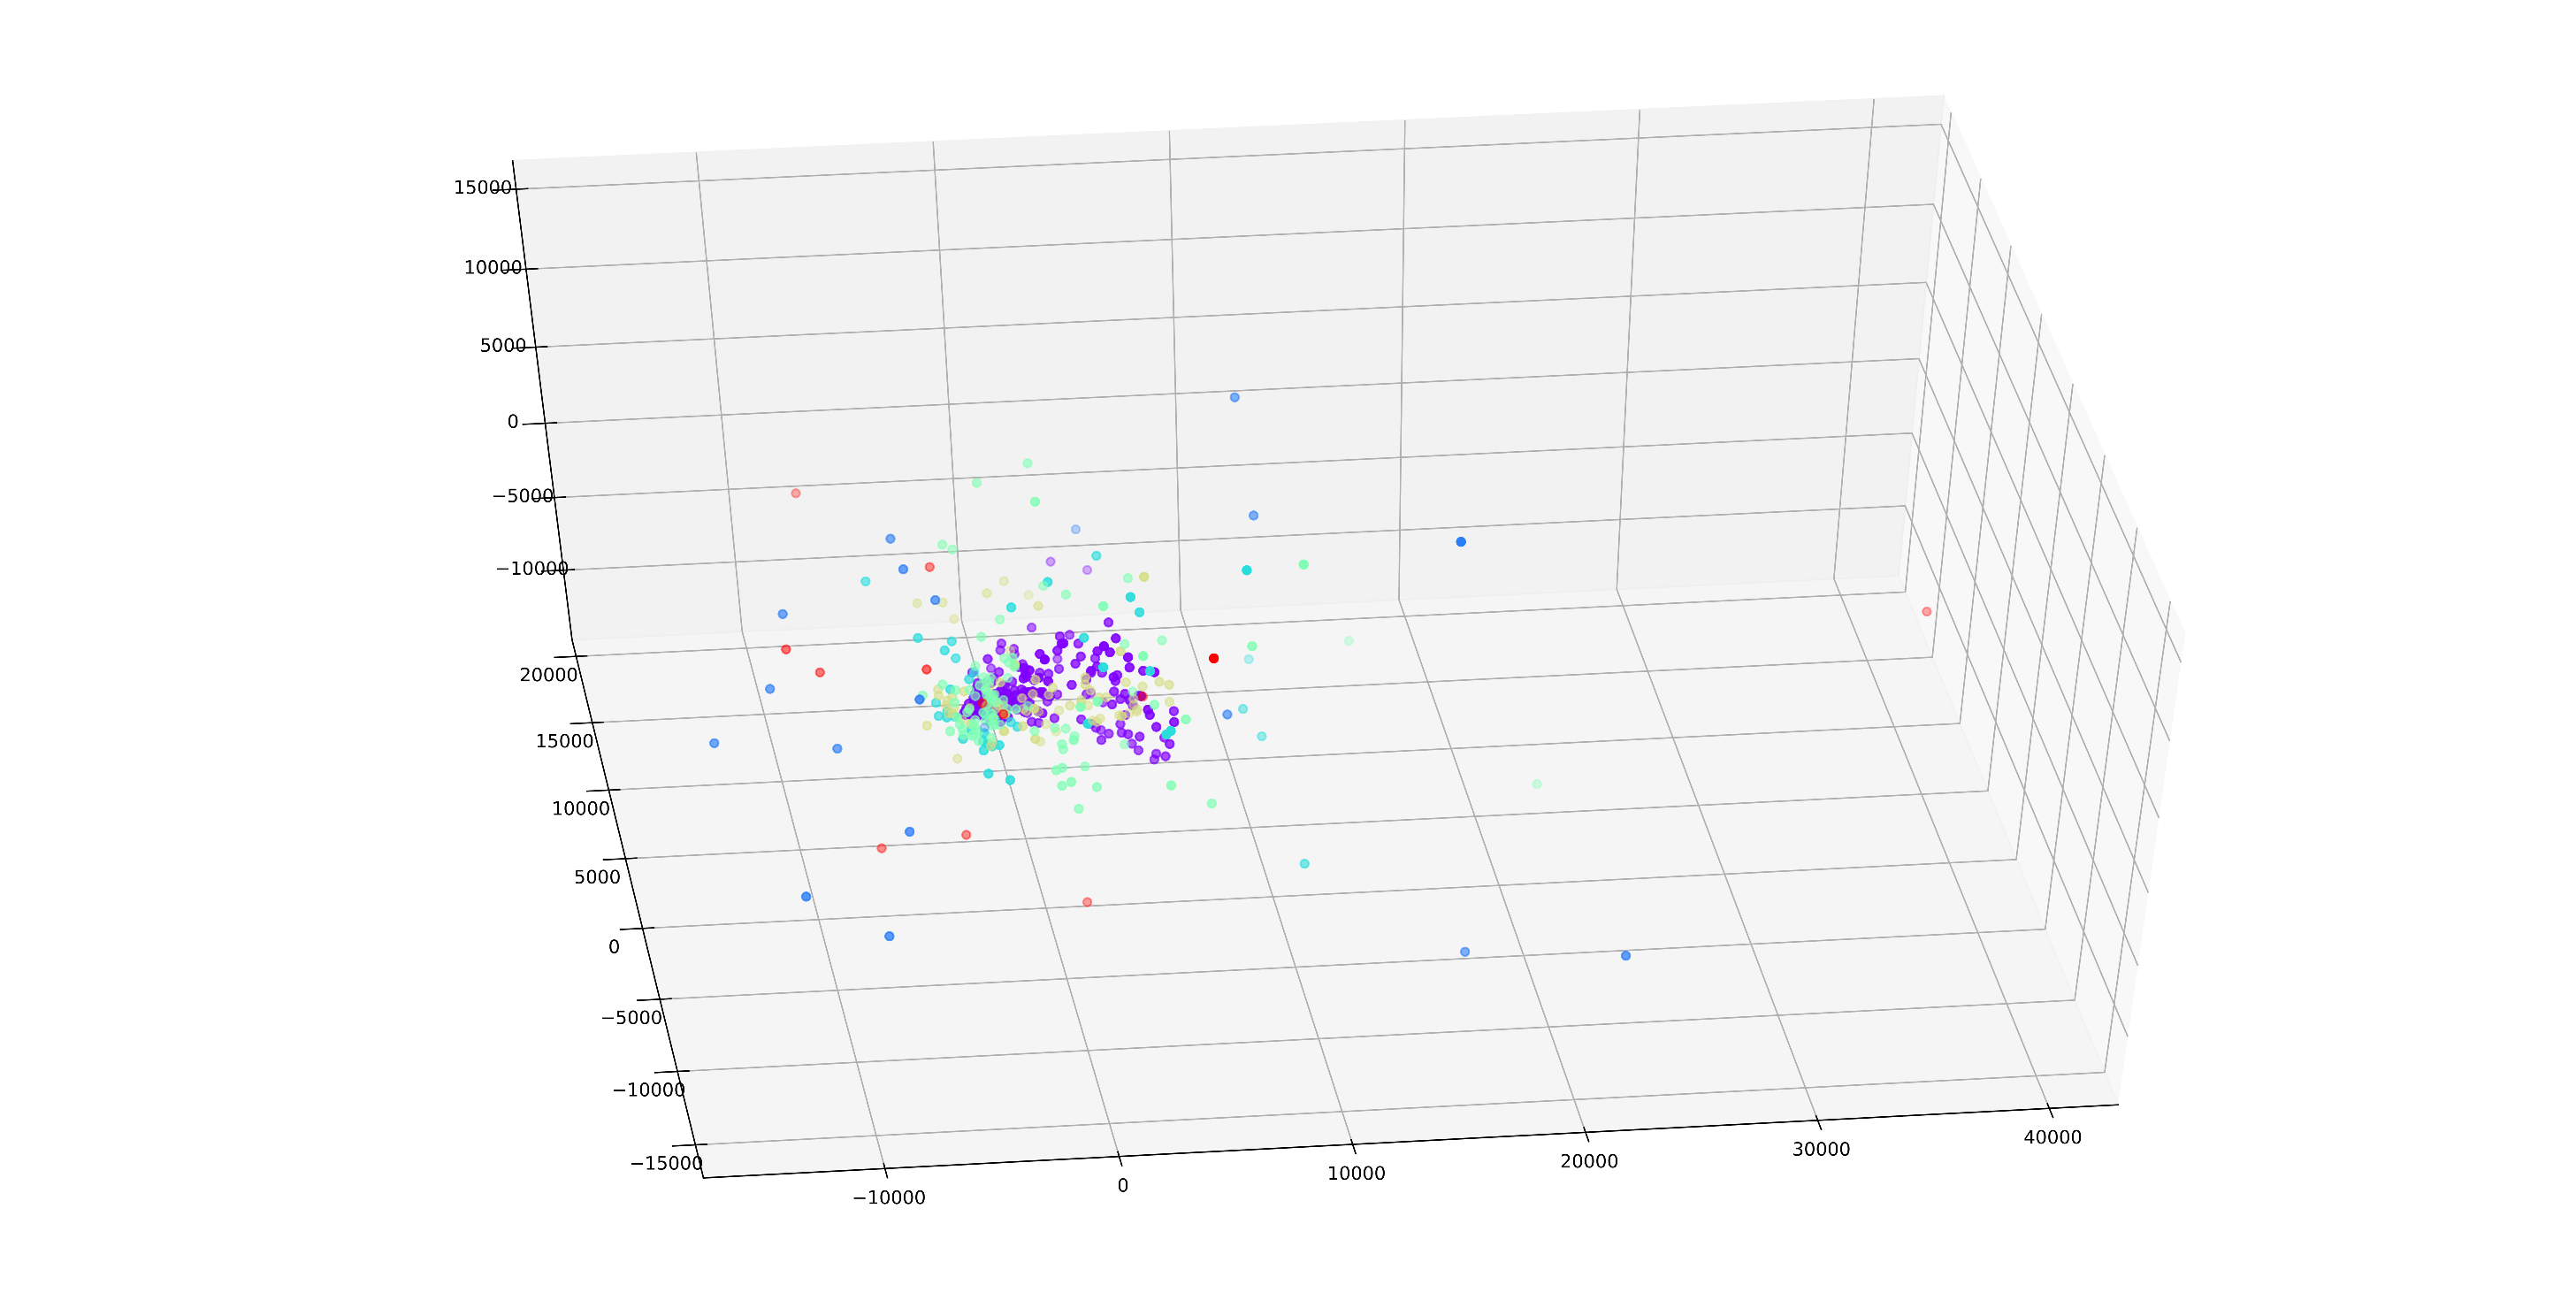
\includegraphics[width=.48\textwidth]{../images/vizualization/kmeans_7_1.eps}}
                    }
                    {
                        \caption{.}\label{fig::kmeans_1}
                    }
                    \ffigbox[\FBwidth]
                    {
                        \fbox{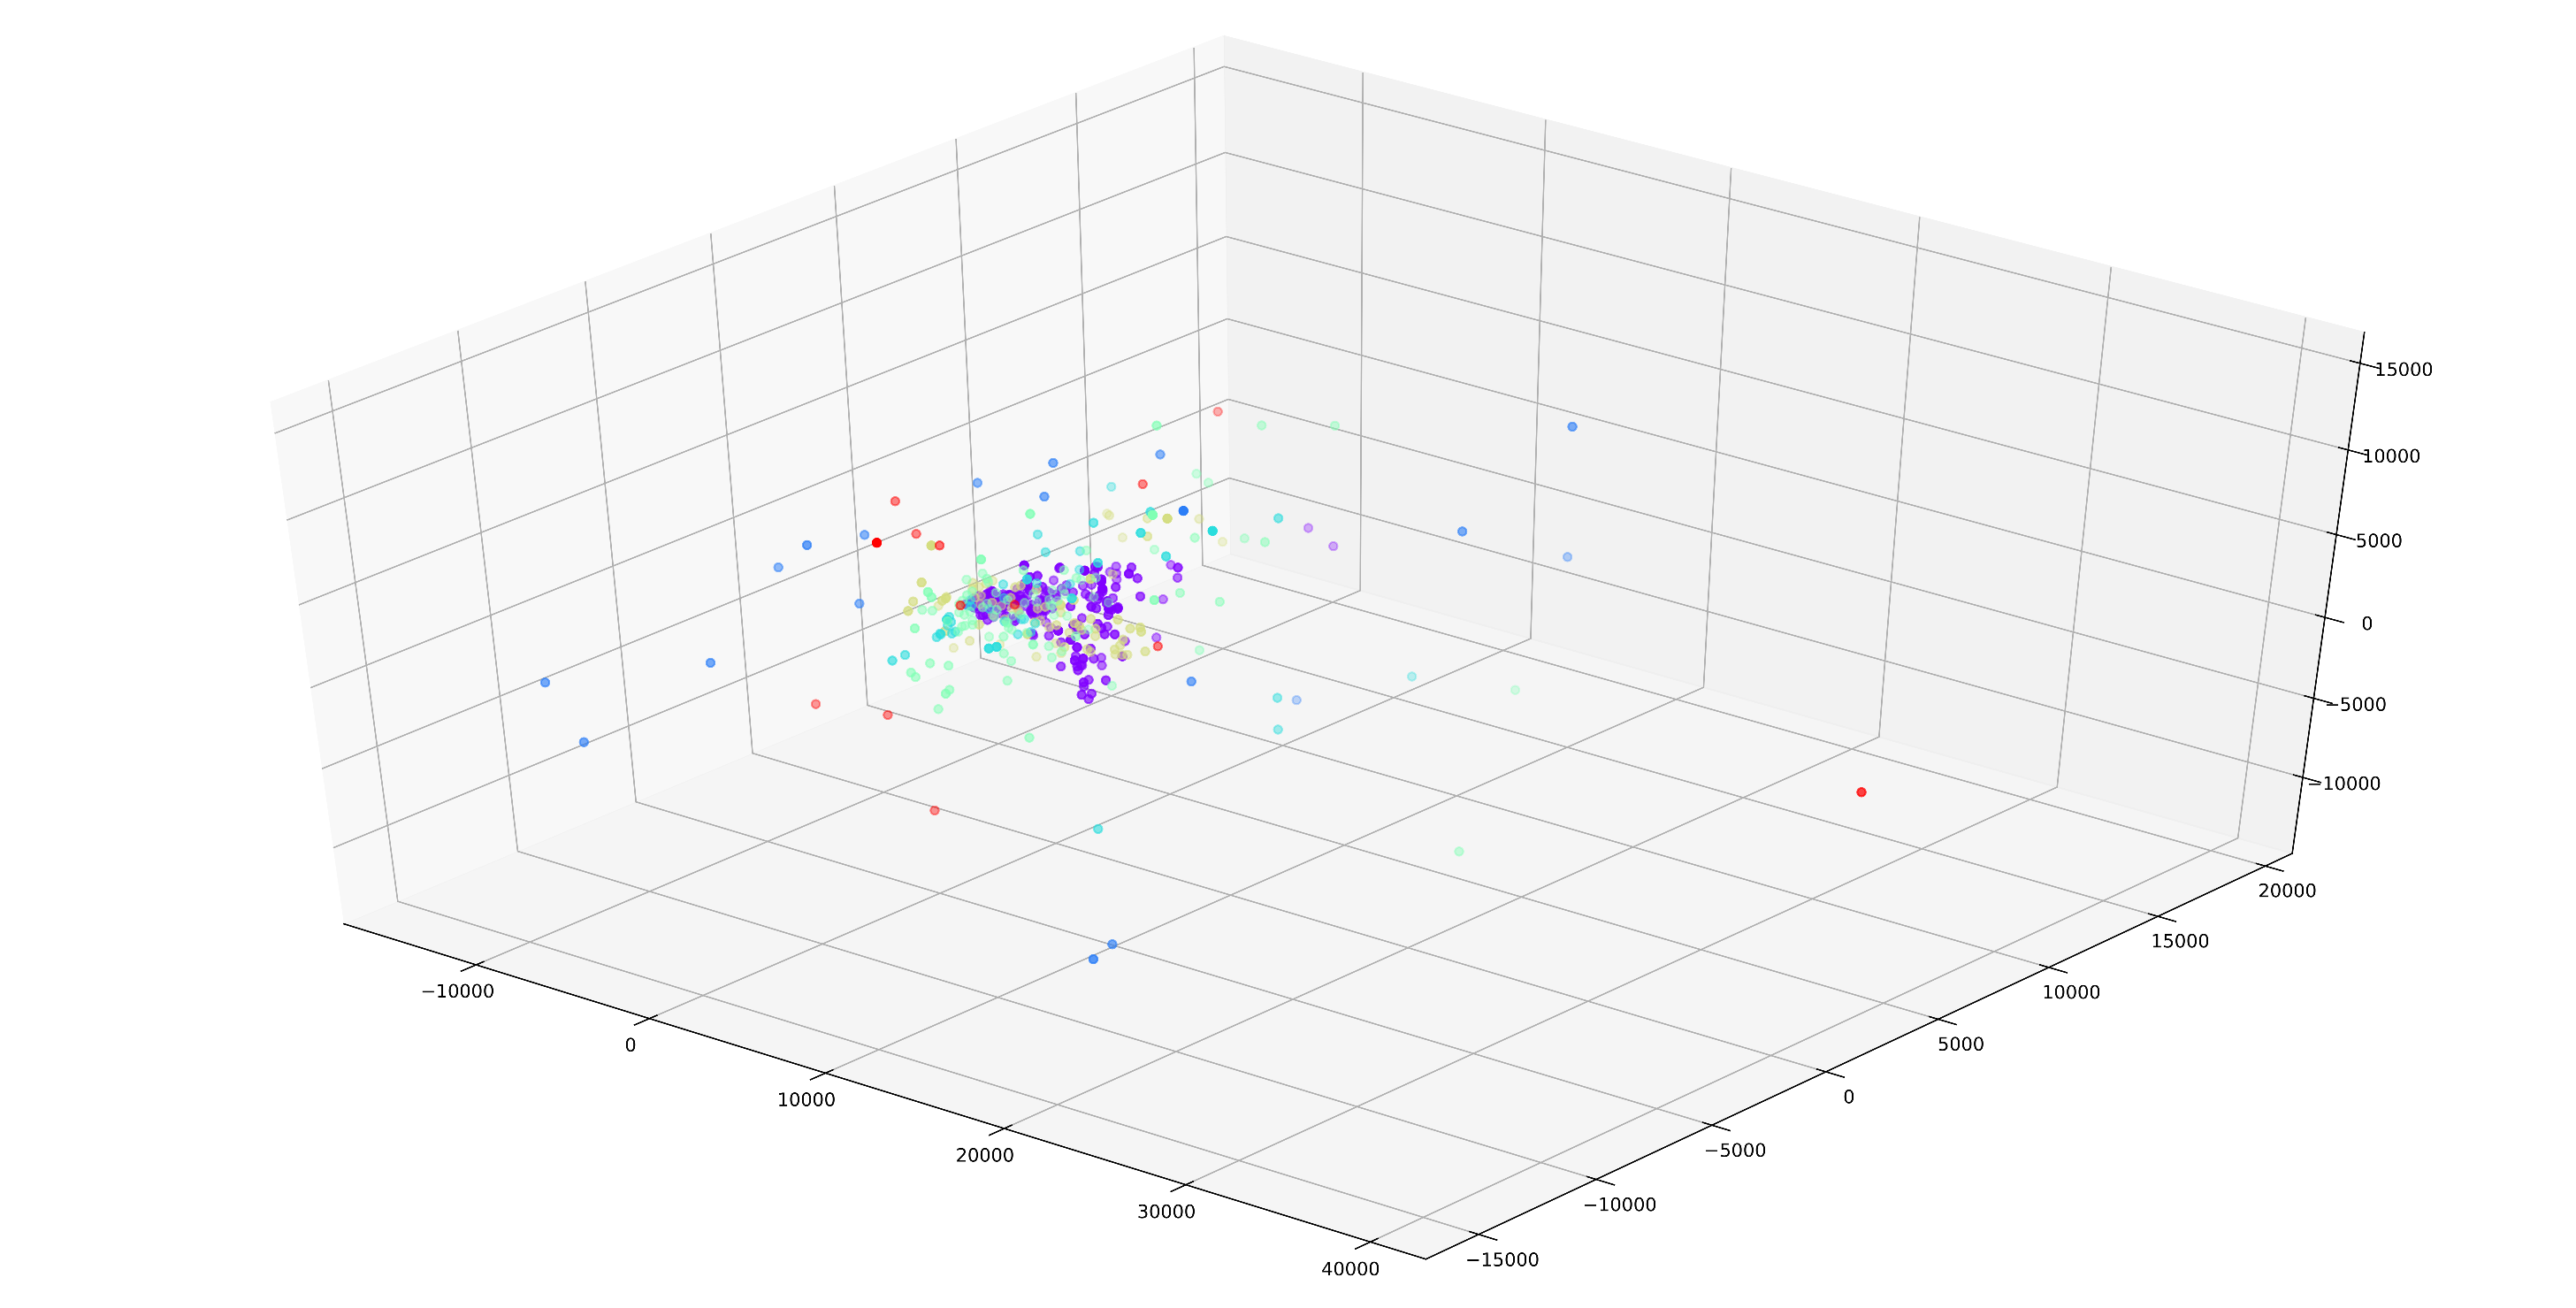
\includegraphics[width=.48\textwidth]{../images/vizualization/kmeans_7_2.eps}}
                    }
                    {
                        \caption{.}\label{fig::kmeans_2}
                    }
                \end{subfloatrow}
            }
            {
                \caption*{(i). Visualization of K-means results.}
            }
            \ffigbox[\FBwidth]
            {
                \begin{subfloatrow}[2]
                    \captionsetup{labelformat=brace, justification=raggedright}
                    \ffigbox[\FBwidth]
                    {
                        \fbox{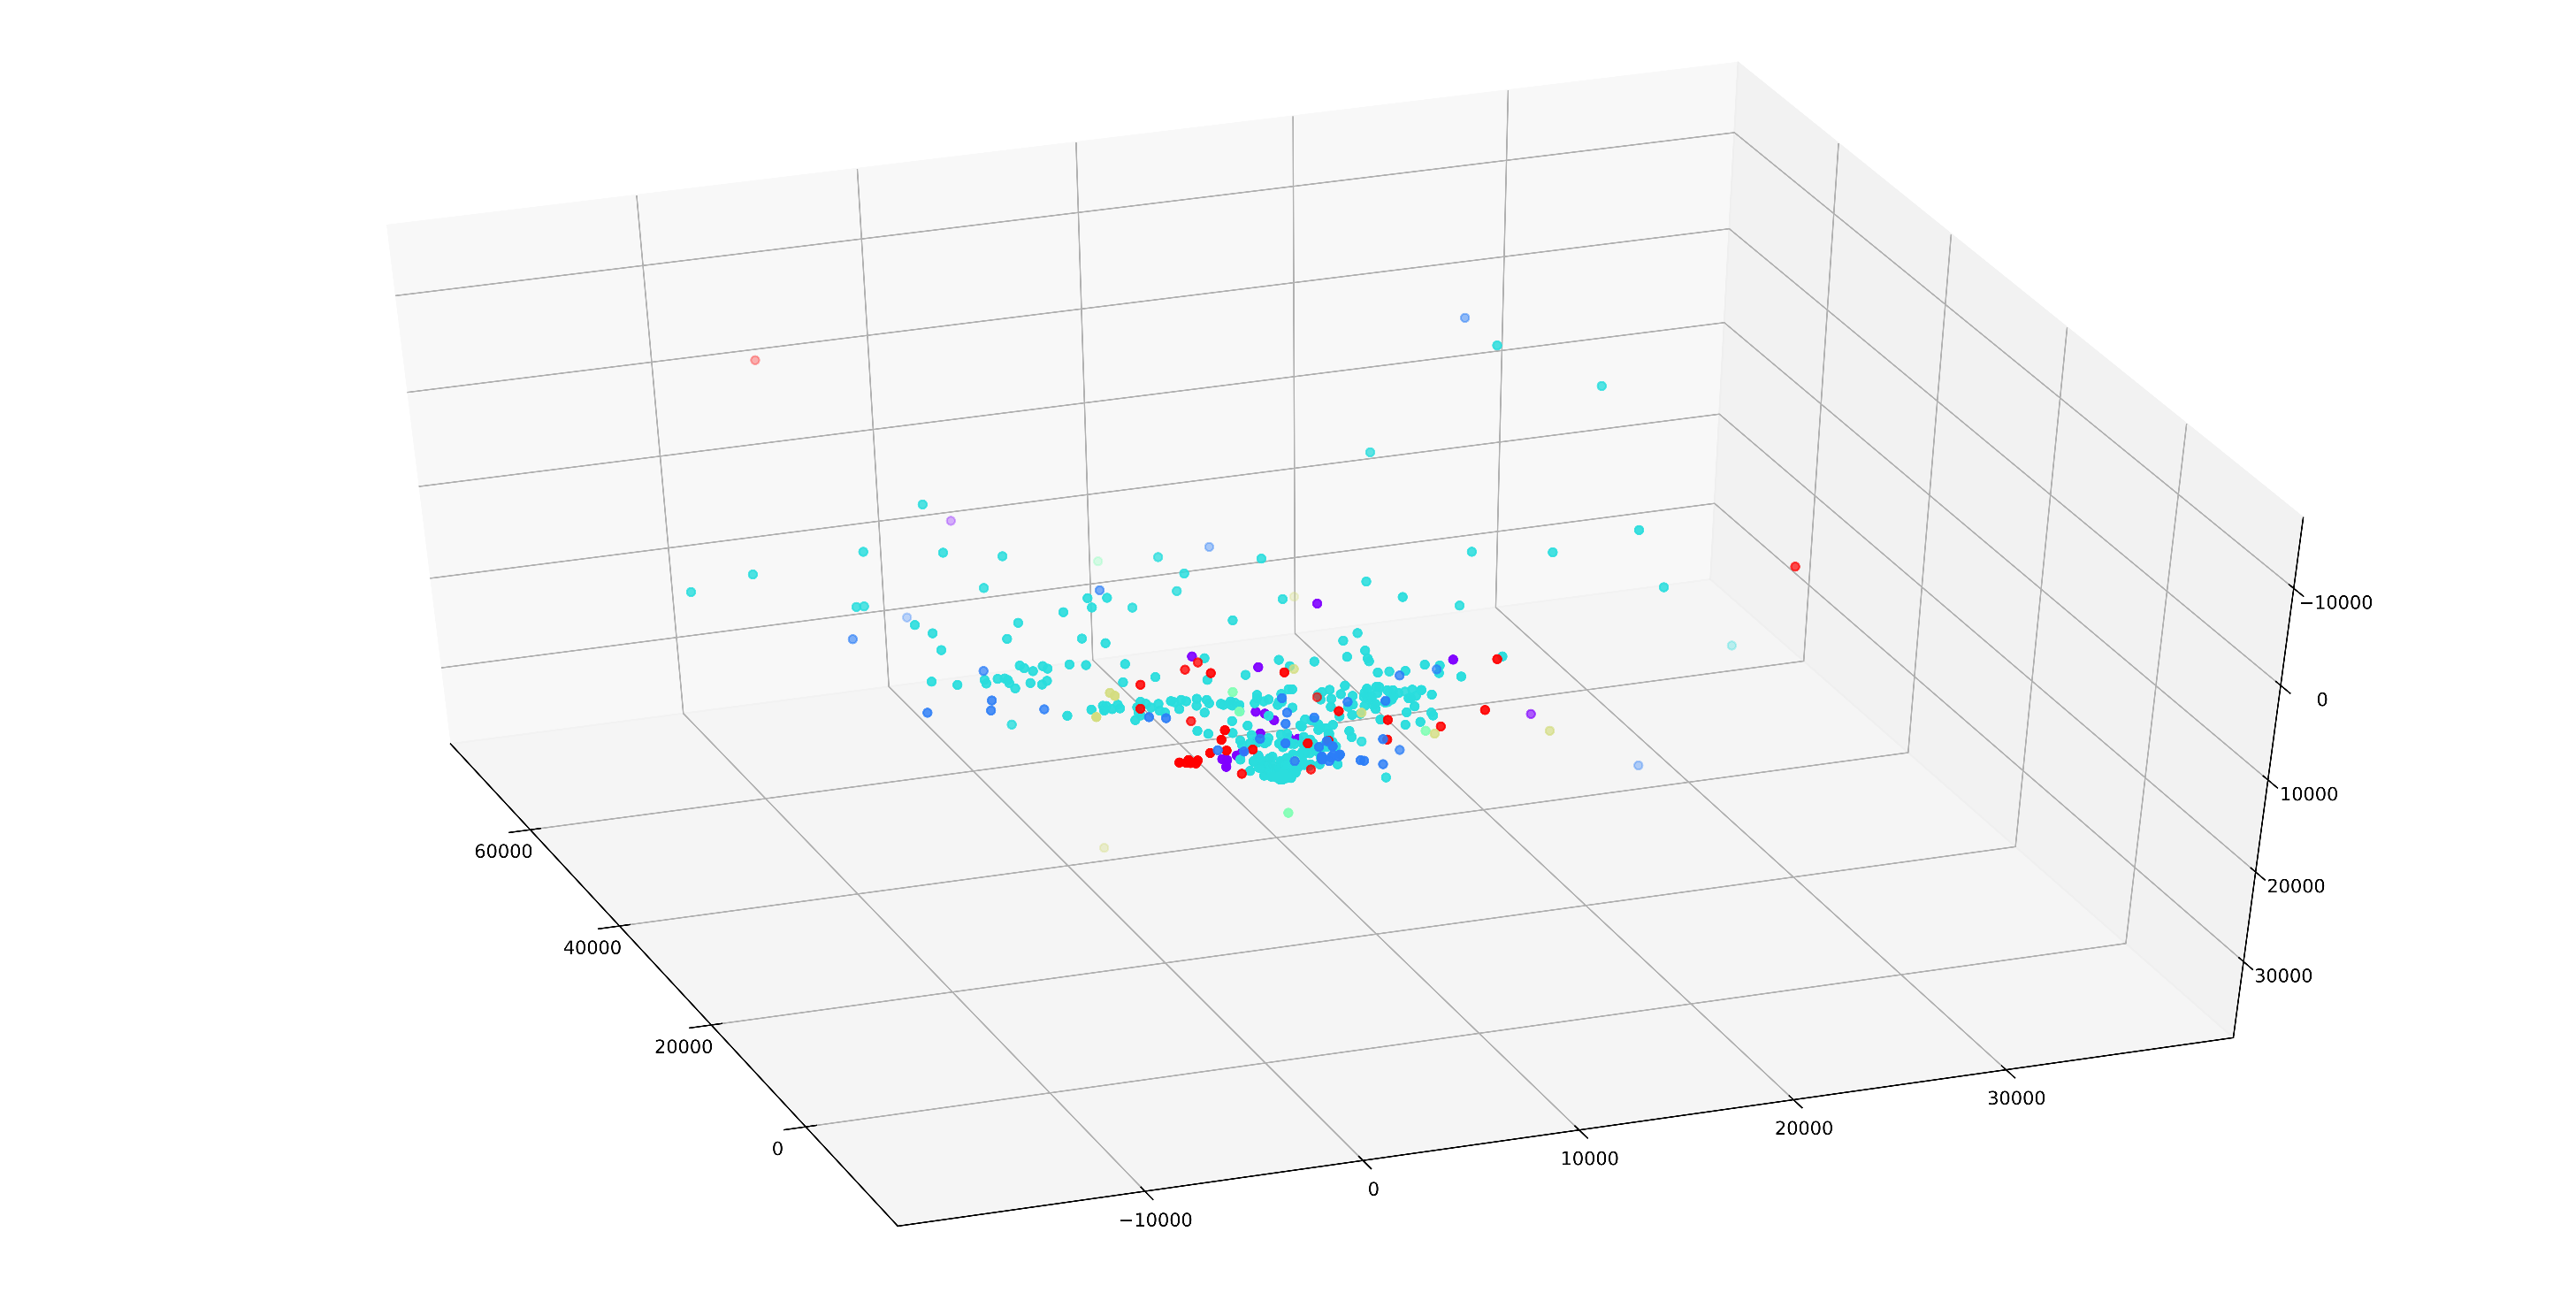
\includegraphics[width=.48\textwidth]{../images/vizualization/spectral_clus_7_1.eps}}
                    }
                    {
                        \caption{.}\label{fig::spectral_1}
                    }
                    \ffigbox[\FBwidth]
                    {
                        \fbox{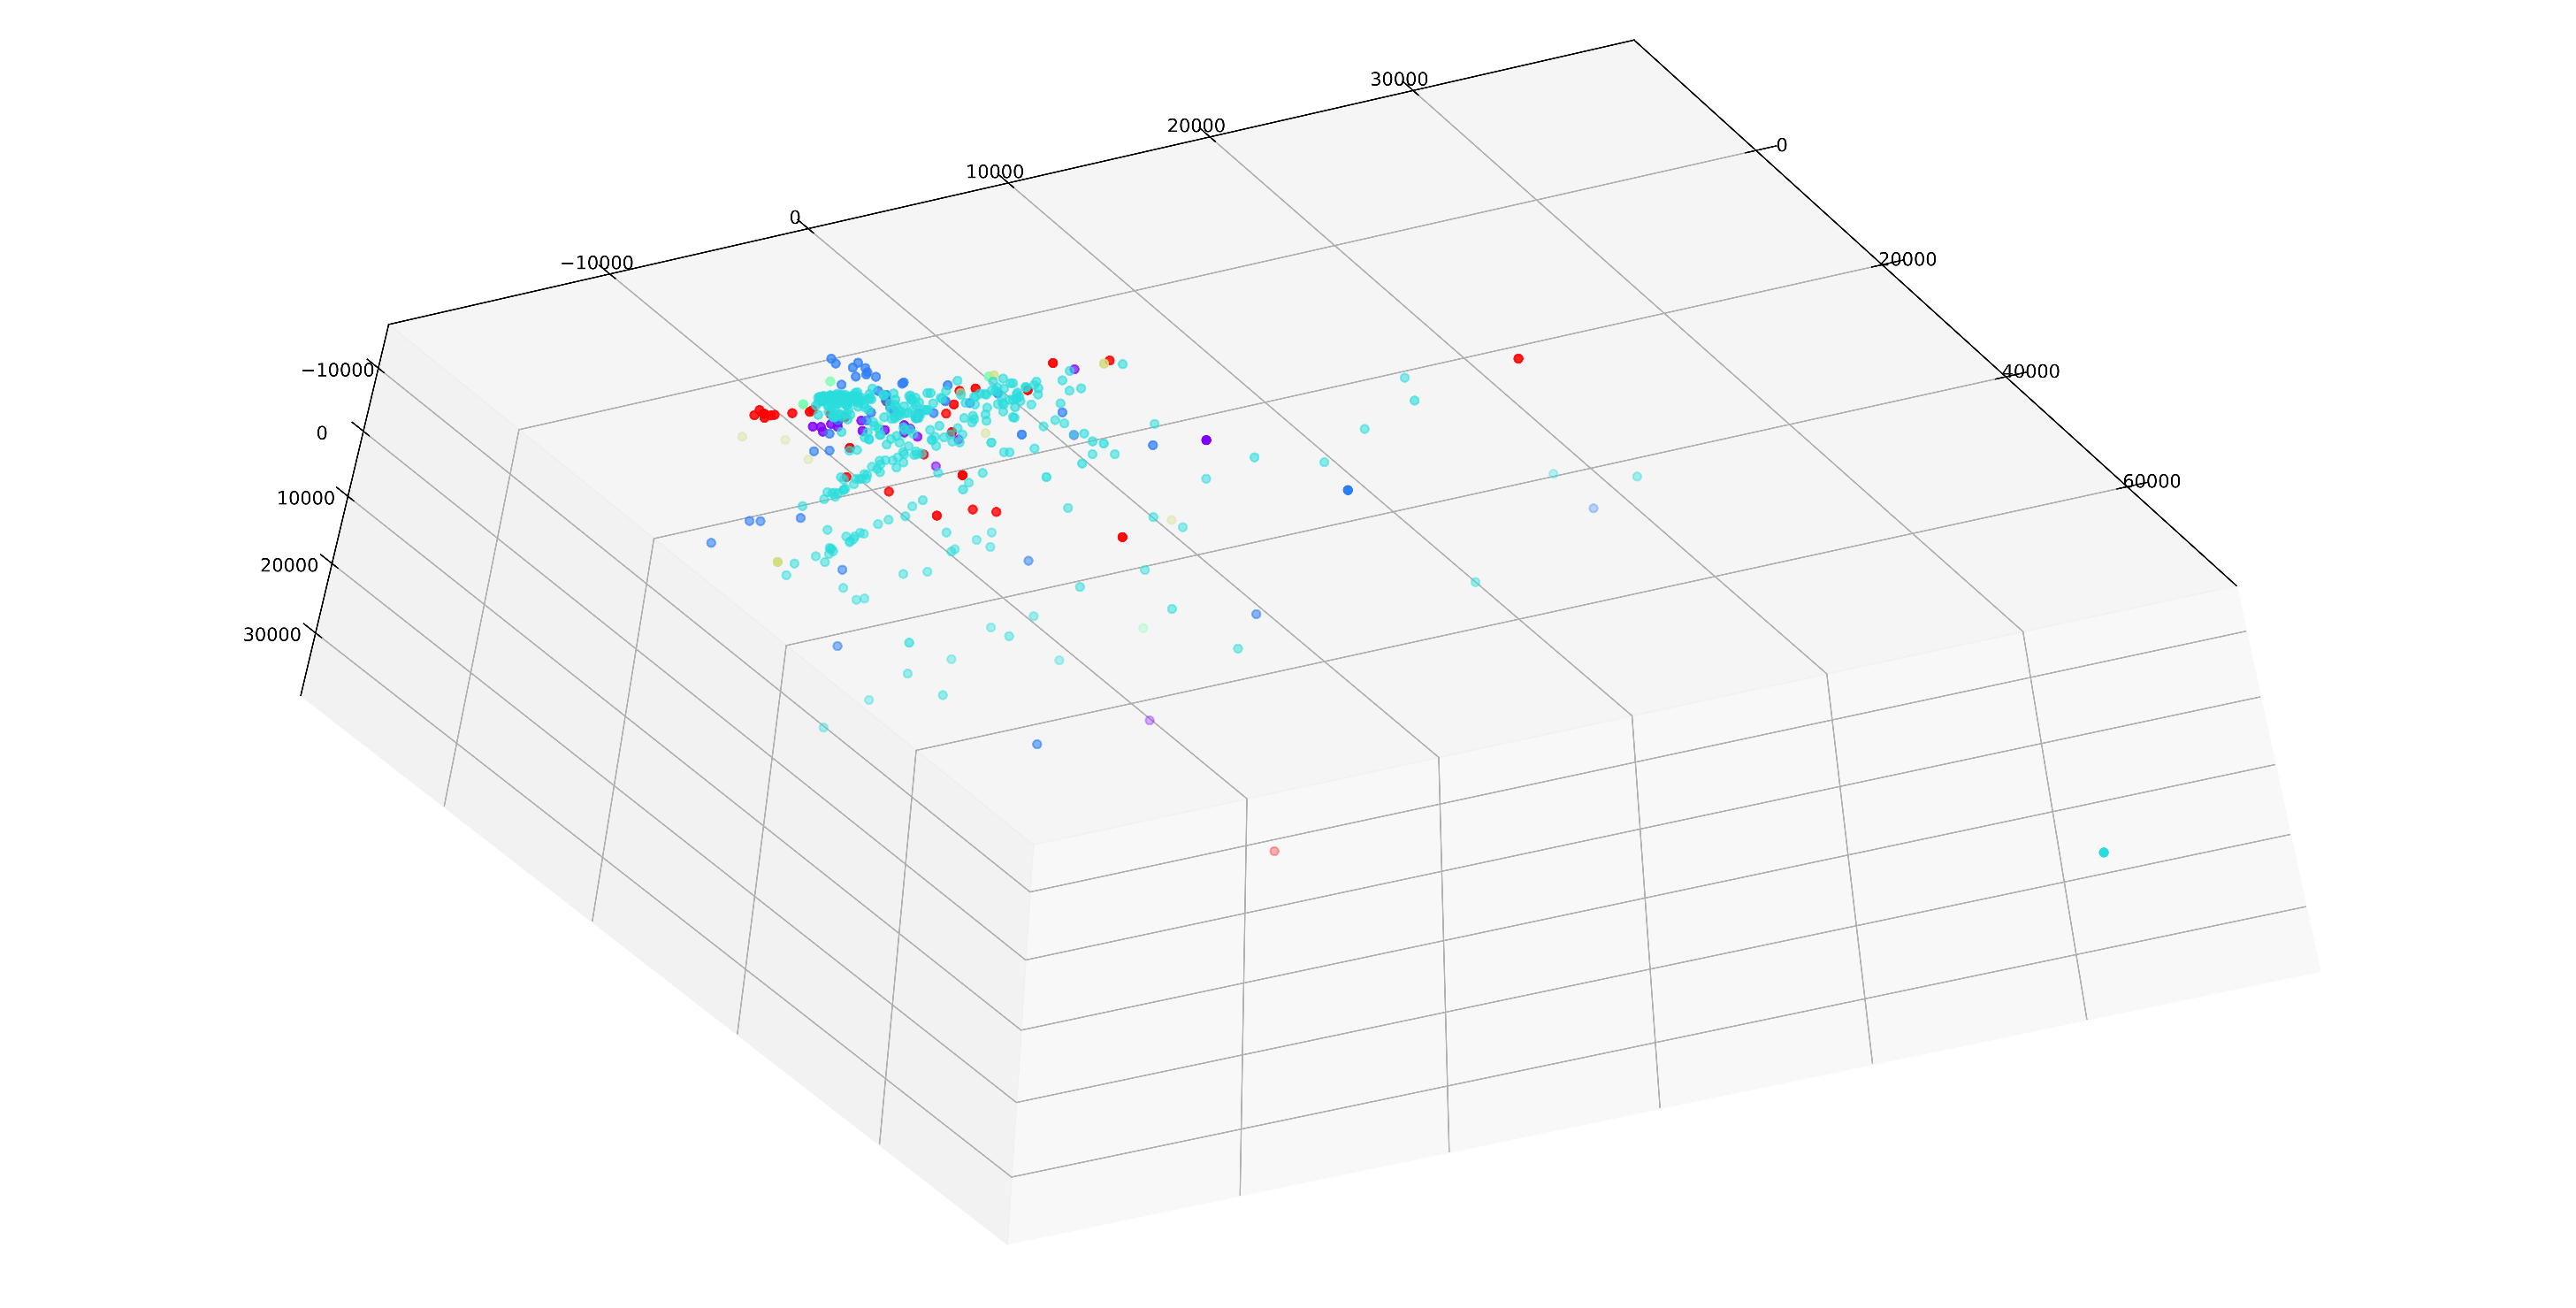
\includegraphics[width=.48\textwidth]{../images/vizualization/spectral_clus_7_2.eps}}
                    }
                    {
                        \caption{.}\label{fig::spectral_2}
                    }
                \end{subfloatrow}
            }
            {
                \caption*{(ii). Visualization of Spectral clustering results.}
            }
        }
        {
            \caption{\label{fig::clust_viz} Visualization of \textit{PCA} reduced clusters: we specified for both methods $7$ clusters.}
        }
    \end{figure}

    \subsection{Classification results}

    The classification pipeline is subdivided into two phases:

    \begin{itemize}
        \item[(i).] Binary classification: the idea is to use geometric features to predict the unqualified builings which are to be discarded. They cannot be classified and can be determined by the operator. We site in Table~\ref{tab::binary_rf_1000_4} the results of a $10$-fold cross validation using Random Forests as a classifier with $1000$ trees and $4$ in deepth.

        \item[(ii).] Coarse Multi classification: classifies qualified buildings by the error classes: `None', `Building error', `Facet error'. We can observe the results of cross validated \textit{Random Forests} and \textit{SVM} in Figure~\ref{fig::class_viz}. We can also observe how facet relations play a big role in the classification in Figure~\ref{fig::feat_import}.
    \end{itemize}

    \begin{table}[H]
        \caption{\label{tab::binary_rf_1000_4}Binary classification results using a Random Forests (trees: $1000$, depth: $4$).}
        \begin{tabular}{c c c}
            \toprule
             & \textbf{Unqualified buildings} & \textbf{Qualified models} \\
            \midrule
            Class statistics & $11.55$\% & $88.45$\% \\
            \midrule
            \midrule
            \multicolumn{3}{c}{\textbf{Cross validation results}}\\
            \midrule
            Metric & Max & Min \\
             \midrule
            train scores & $1.000$ & $0.9911$ \\
             \midrule
            fit time & $1.779$ secs & $1.693$ secs \\
             \midrule
            test scores & $1.000$ & $0.8775$\\
             \midrule
            score time & $0.2507$ secs & $0.2020$ secs\\
             \bottomrule
        \end{tabular}
    \end{table}

    \begin{figure}[H]
        \ffigbox{
            \ffigbox[\FBwidth]{
                \begin{subfloatrow}[1]
                    \captionsetup{labelformat=brace, justification=raggedright}
                        \fbox{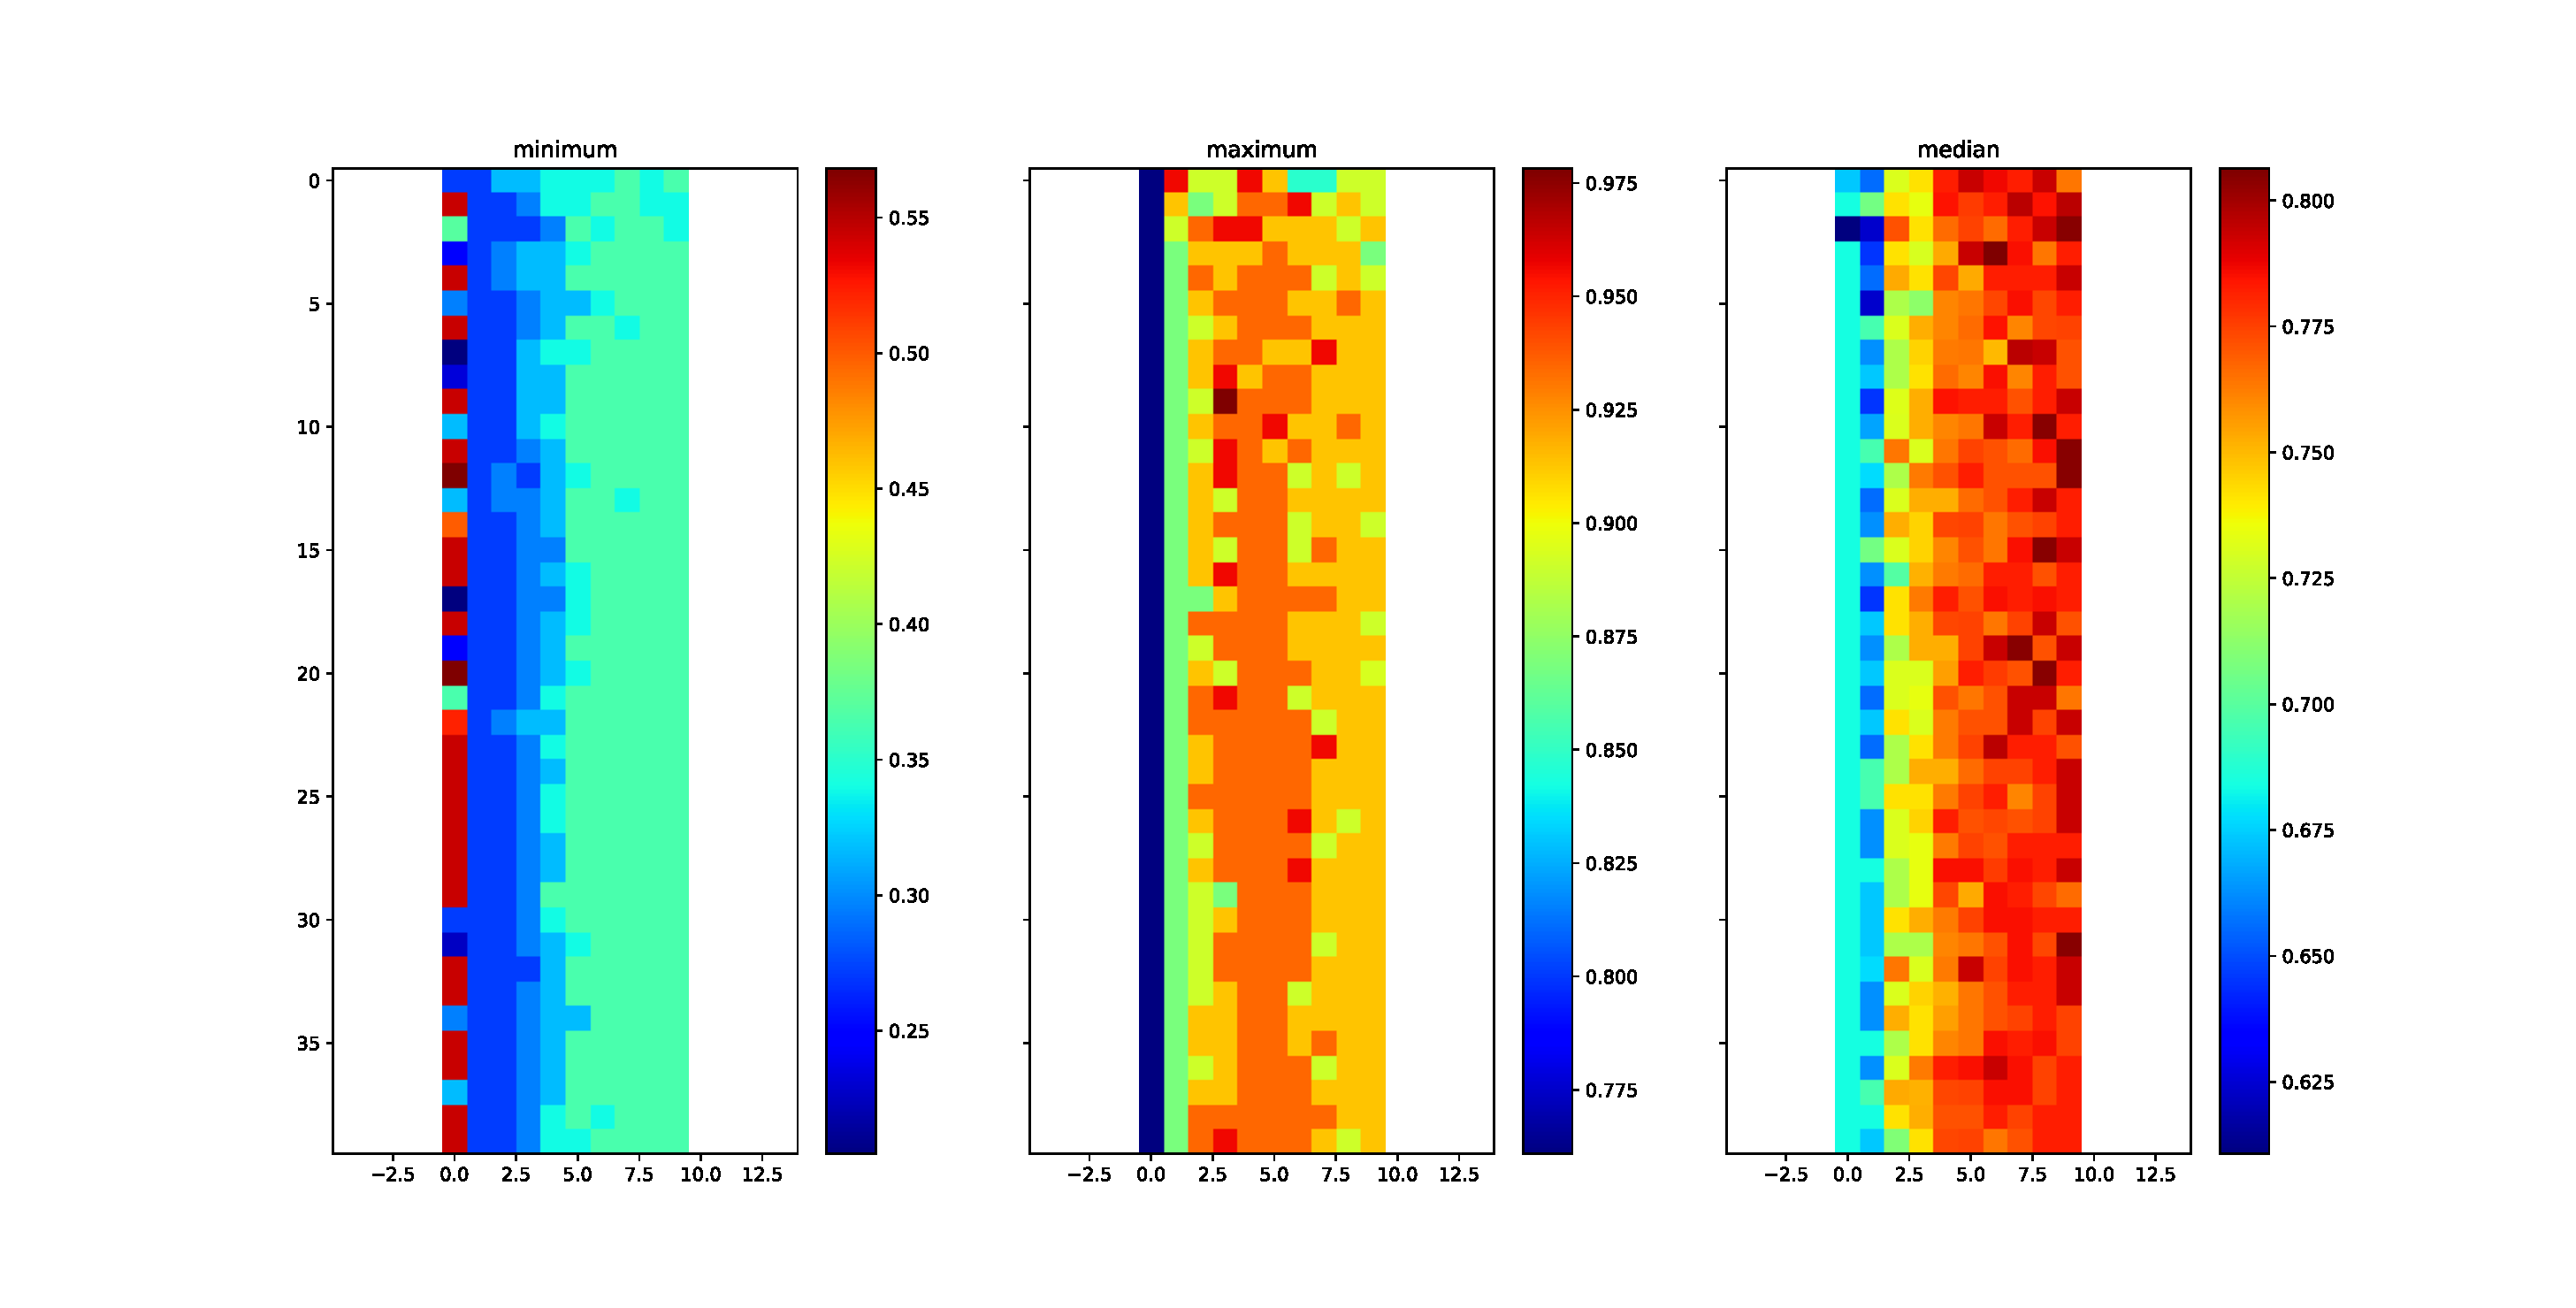
\includegraphics[width=.75\textwidth]{../images/classification/rf_geom_depth_nbr50}}
                \end{subfloatrow}
            }
            {
                \caption*{(i). Visualization of \textit{Random Forest} results on geometric features.}
            }
            \ffigbox[\FBwidth]{
                \begin{subfloatrow}[1]
                    \captionsetup{labelformat=brace, justification=raggedright}
                        \fbox{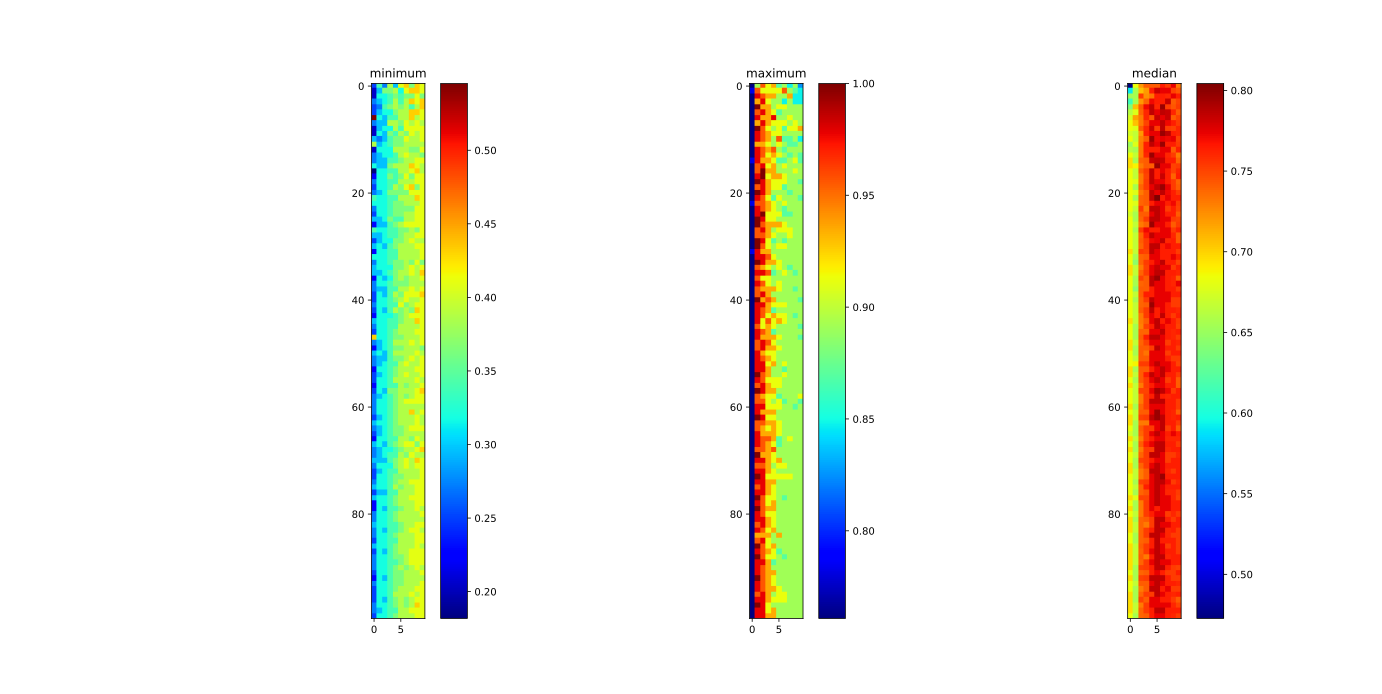
\includegraphics[width=.75\textwidth]{../images/classification/rf_geom_altim_depth_nbr25}}
                \end{subfloatrow}
            }
            {
                \caption*{(ii). Visualization of \textit{Random Forest} results on fused features.}
            }
            \ffigbox[\FBwidth]{
                \begin{subfloatrow}[1]
                    \captionsetup{labelformat=brace, justification=raggedright}
                        \fbox{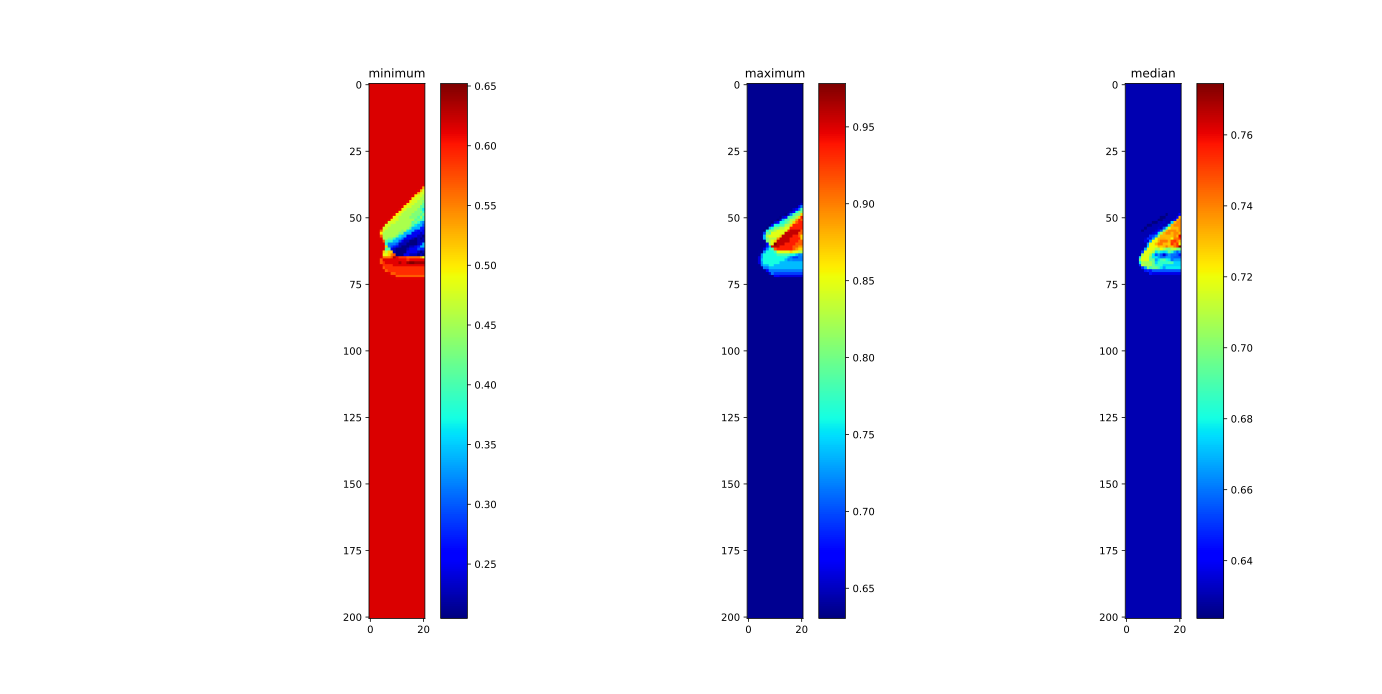
\includegraphics[width=.75\textwidth]{../images/classification/svm_C10pgo5_20_gamma_10pgo5_200}}
                \end{subfloatrow}
            }
            {
                \caption*{(iii). Visualization of \textit{SVM} results.}
            }
        }
        {
            \caption{\label{fig::class_viz} Visualization of Cross validated coarse classification scores.}
        }
    \end{figure}

    \begin{figure}[H]
        \ffigbox[\FBwidth]{
            \begin{subfloatrow}[1]
                \captionsetup{labelformat=brace, justification=raggedright}
                \fbox{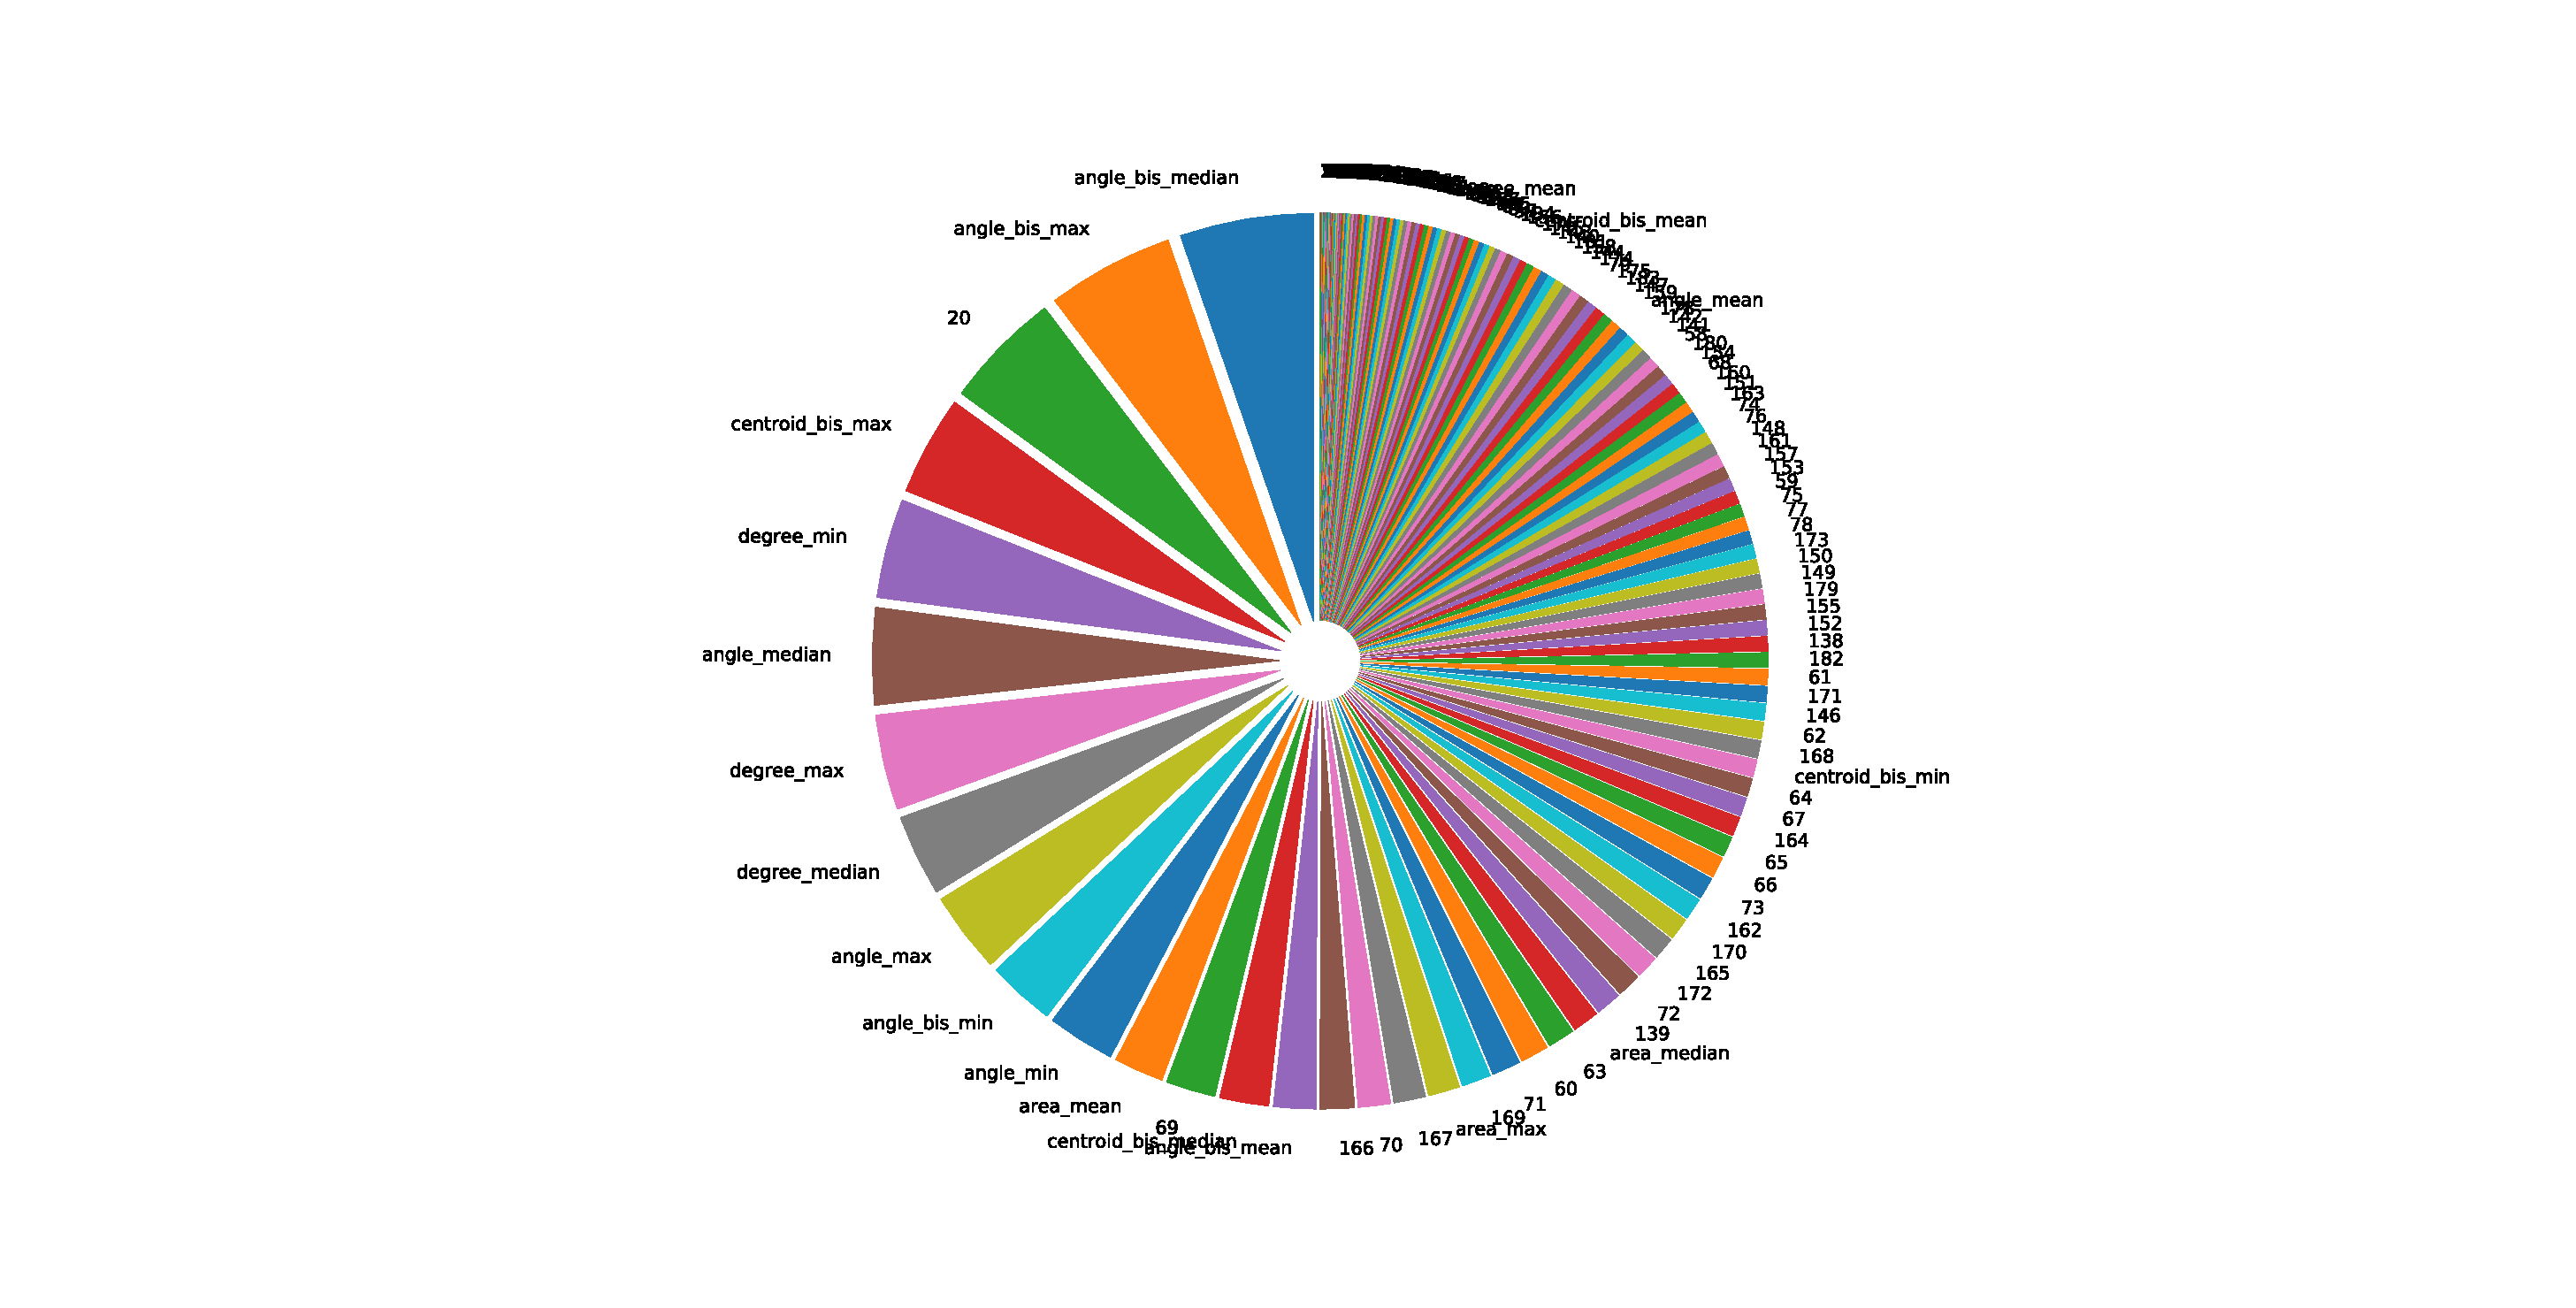
\includegraphics[width=.75\textwidth]{../images/classification/feat_importance_rf}}
            \end{subfloatrow}
        }
        {
            \caption{\label{fig::feat_import} Pie chart visualizing feature importance.}
        }
    \end{figure}

    We need to classify now on subclasses and try to link the results back to real building in QGIS\@.
\end{document}
